\chapter{Implementasi dan Evaluasi}

\section{Hasil Eksplorasi CARLA}

Setelah membaca dokumentasi CARLA dan mengeksplorasi CARLAUE4 diketahui terdapat
beberapa fitur sebagai berikut:

\begin{enumerate}
	\item Penambahan kendaraan baru beroda empat dan dua.
	\item Penambahan \textit{spline} untuk menambahkan rel.
	\item Penambahan objek statis lainnya.
\end{enumerate}

% dapat dilakukan implementasi kendaraan roda 4, 2
% dapat dilakukan implementasi rel menggunakan spline (add ref?)
% dapat dilakukan implementasi objek statis

% TODO: ? cara import aset yang lain (yang khusus, yang detail di bawah aja)
% TODO: ? BP, factory, spline
% TODO: jelasin how to? but where

\section{Implementasi Trem dan Angkot}

\subsection{Pembuatan Aset Model 3D untuk Ekspor FBX}

Implementasi trem dan angkot mengikuti langkah-langkah pada
\cite{blender-add-a-new-vehicle}. Pembuatan \textit{mesh} model 3D perlu sesuai
dengan persyaratan dari CARLA, yaitu jumlah tris (segitiga satuan yang membentuk
permukaan) 50.000-100.000, melakukan pemisahan material/tekstur sesuai dengan
bagian kendaraan agar tampilan sesuai saat disimulasikan.

Setelah model 3D dibuat, aset \textit{vehicle skeleton} atau \textit{armature}
dari \cite{blender-add-a-new-vehicle} perlu ditambahkan, diatur posisi
\textit{bone} dari \textit{armature}, dan dihubungkan ke \textit{mesh} model 3D.
Gambar \ref{fig:vehicle-skeleton} menunjukkan aset yang harus ditambahkan pada
kendaraan. Setelah \textit{armature} ditambahkan, masing-masing \textit{head}
dari \textit{bone} roda perlu diposisikan di tengah ban (lihat Gambar
\ref{fig:armature-placement}). Aset \textit{armature} hanya boleh ditranslasi
dan tidak untuk dirotasi ataupun diskala karena akan merusak proses impor
nantinya.

\begin{figure}[ht]
	\centering
	\subfloat[\textit{Vehicle skeleton}]{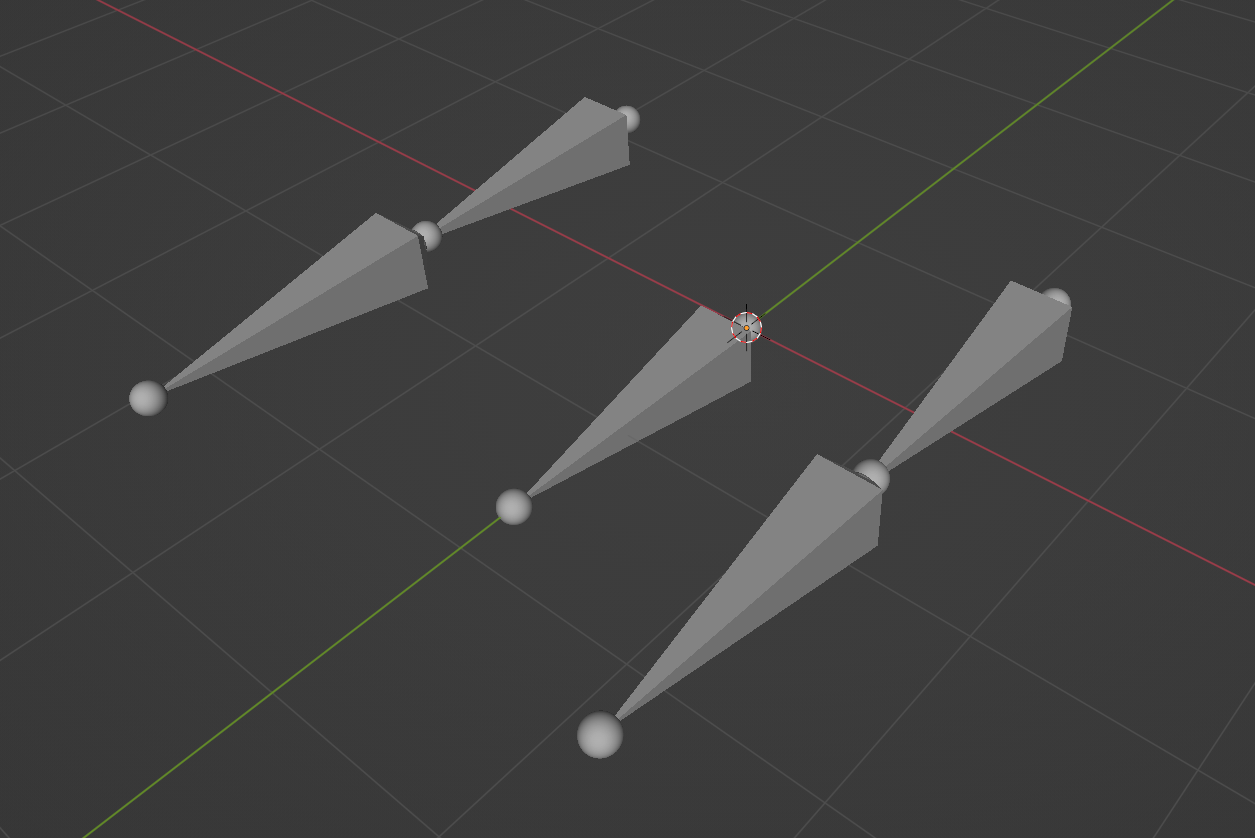
\includegraphics[width=0.4\textwidth]{resources/chapter-4/vehicle-skeleton.png}}
	\hfill
	\subfloat[Hierarki \textit{Vehicle skeleton}]{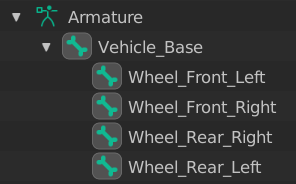
\includegraphics[width=0.4\textwidth]{resources/chapter-4/vehicle-skeleton-hierarchy.png}}
	\caption{\textit{Vehicle skeleton}}
    \label{fig:vehicle-skeleton}
\end{figure}

\begin{figure}[ht]
	\centering
	\subfloat[Tampak samping roda depan kiri angkot]{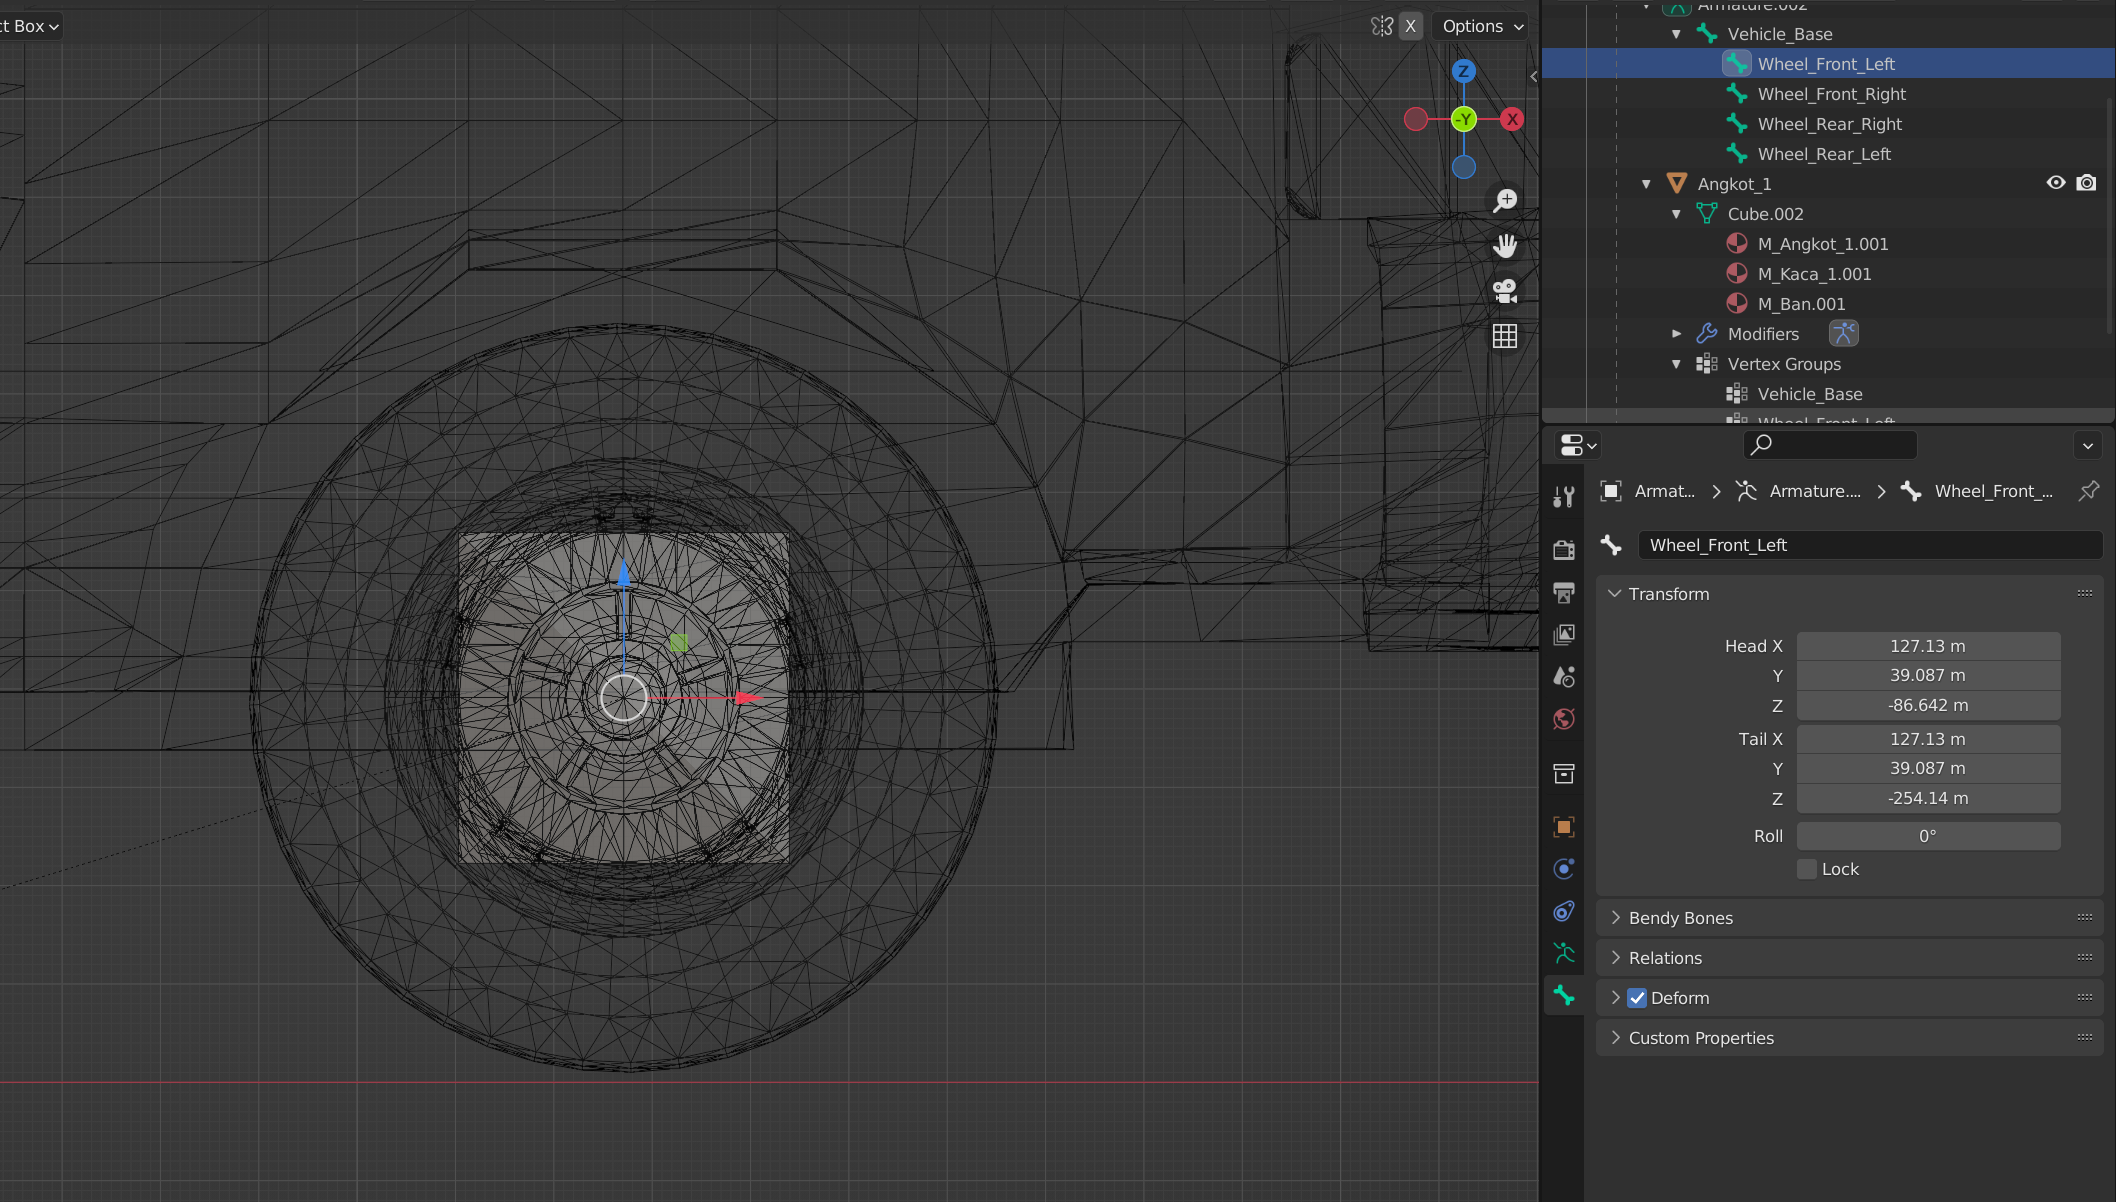
\includegraphics[width=0.4\textwidth]{resources/chapter-4/bone-placement-2.png}}
	\hfill
	\subfloat[Tampak depan roda depan kiri angkot \textit{Vehicle skeleton}]{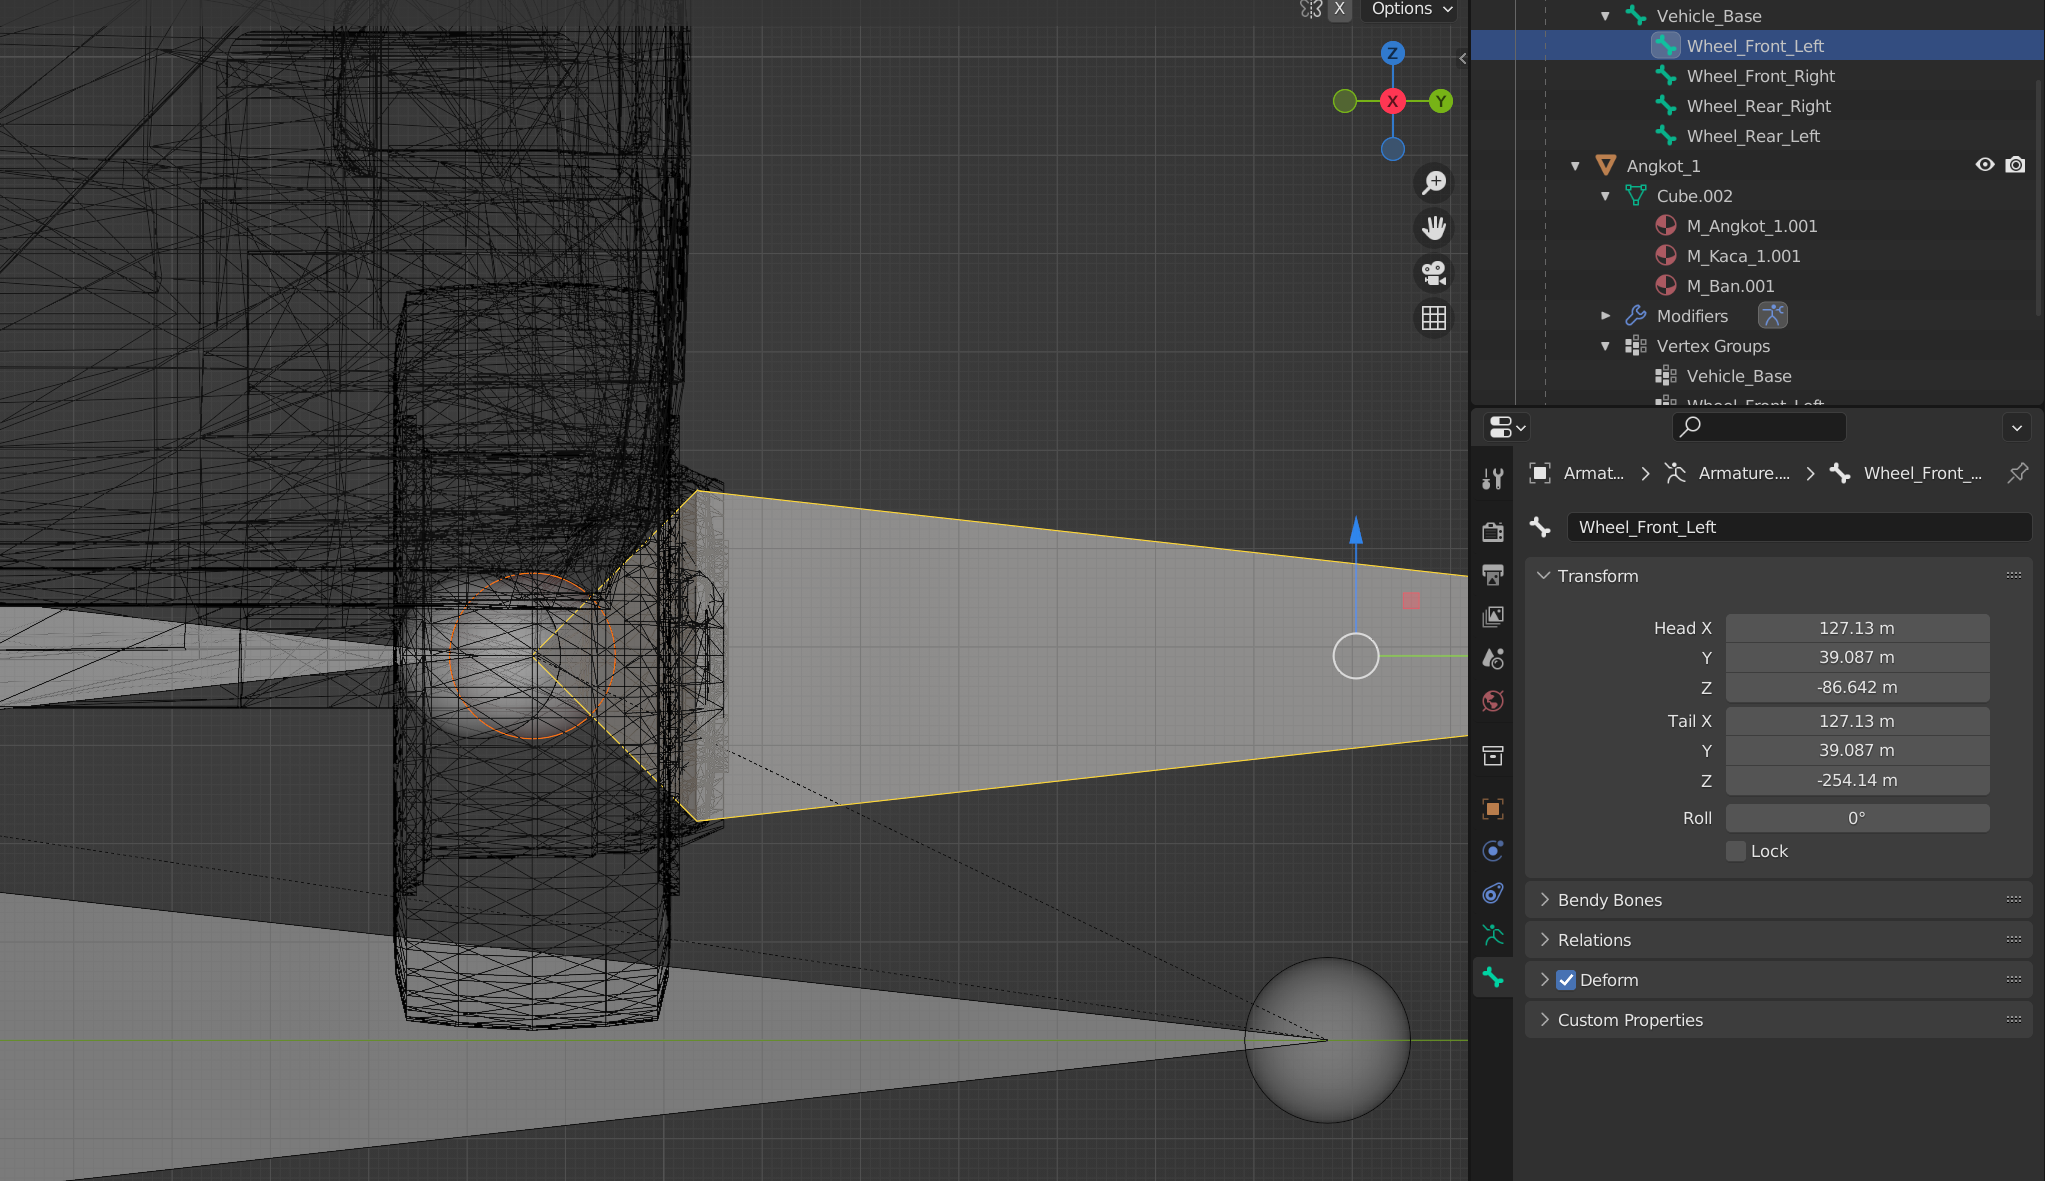
\includegraphics[width=0.4\textwidth]{resources/chapter-4/bone-placement-1.png}}
	\hfill
	\subfloat[Angkot dengan \textit{armature}]{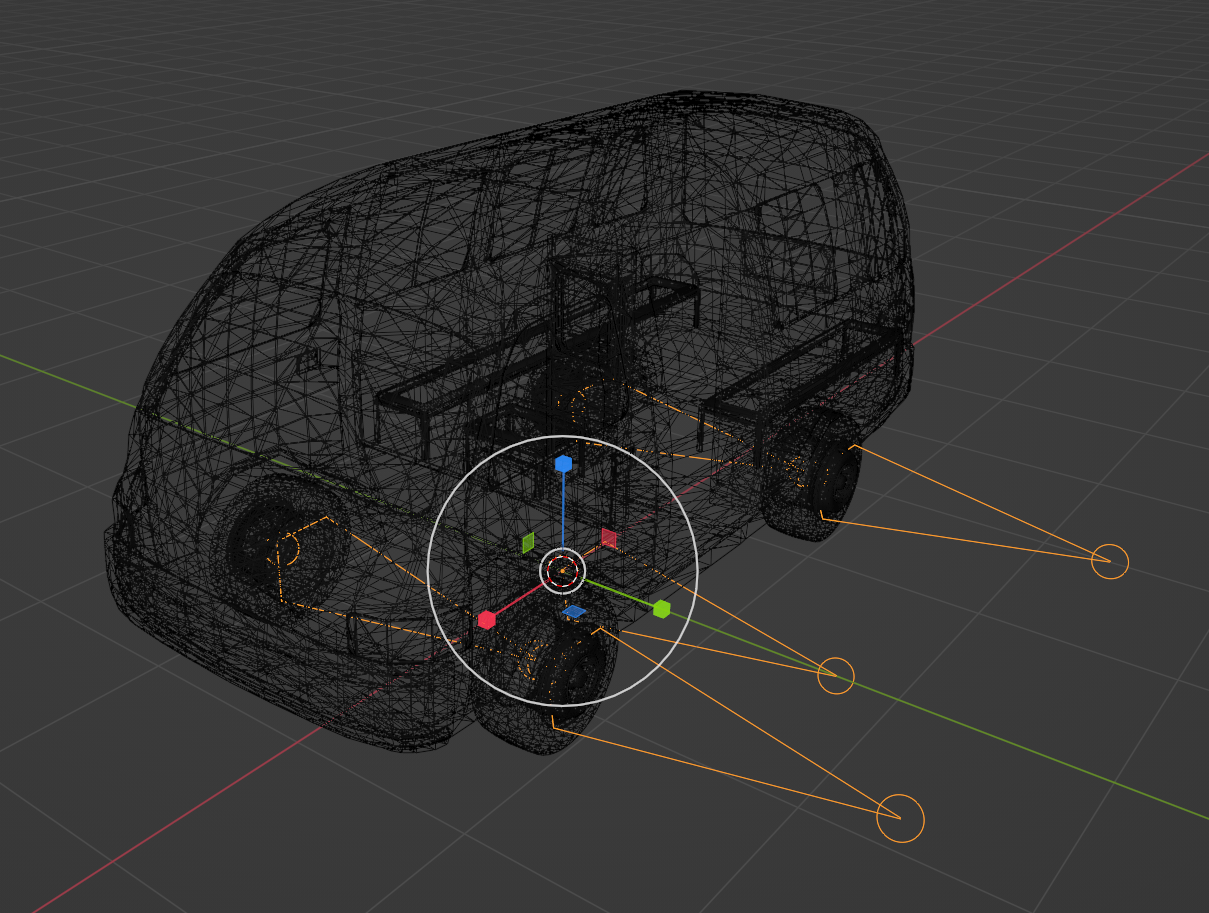
\includegraphics[width=0.4\textwidth]{resources/chapter-4/angkot-model-2.png}}
	\caption{Angkot dengan \textit{Vehicle skeleton} yang sudah di-\textit{skin}}
    \label{fig:armature-placement}
\end{figure}

% TODO: cara skinning di blender
% TODO: cara membuat vertices groups

Setelah semua posisi \textit{bone} sesuai, dilakukan \textit{skinning}
\textit{armature} dengan \textit{mesh} kendaraan. Lima \textit{vertices groups}
dibuat untuk menghubungkan grup-grup dengan \textit{bone} yang sesuai. Kelima
\textit{vertices groups} dibuat dengan nama yang sesuai dengan nama
\textit{bone} yang akan dihubungkan. Gambar \ref{fig:wheel-skinning} menunjukkan
roda angkot bagian depan kiri yang sudah dihubungkan dengan \textit{bone} yang
sesuai. Pengujian ini dilakukan pada \textit{pose mode}, memilih salah satu
\textit{bone}, mengetik 'r', dan menggerakan \textit{cursor}.

\begin{figure}[ht]
	\centering
	\subfloat[Roda posisi awal]{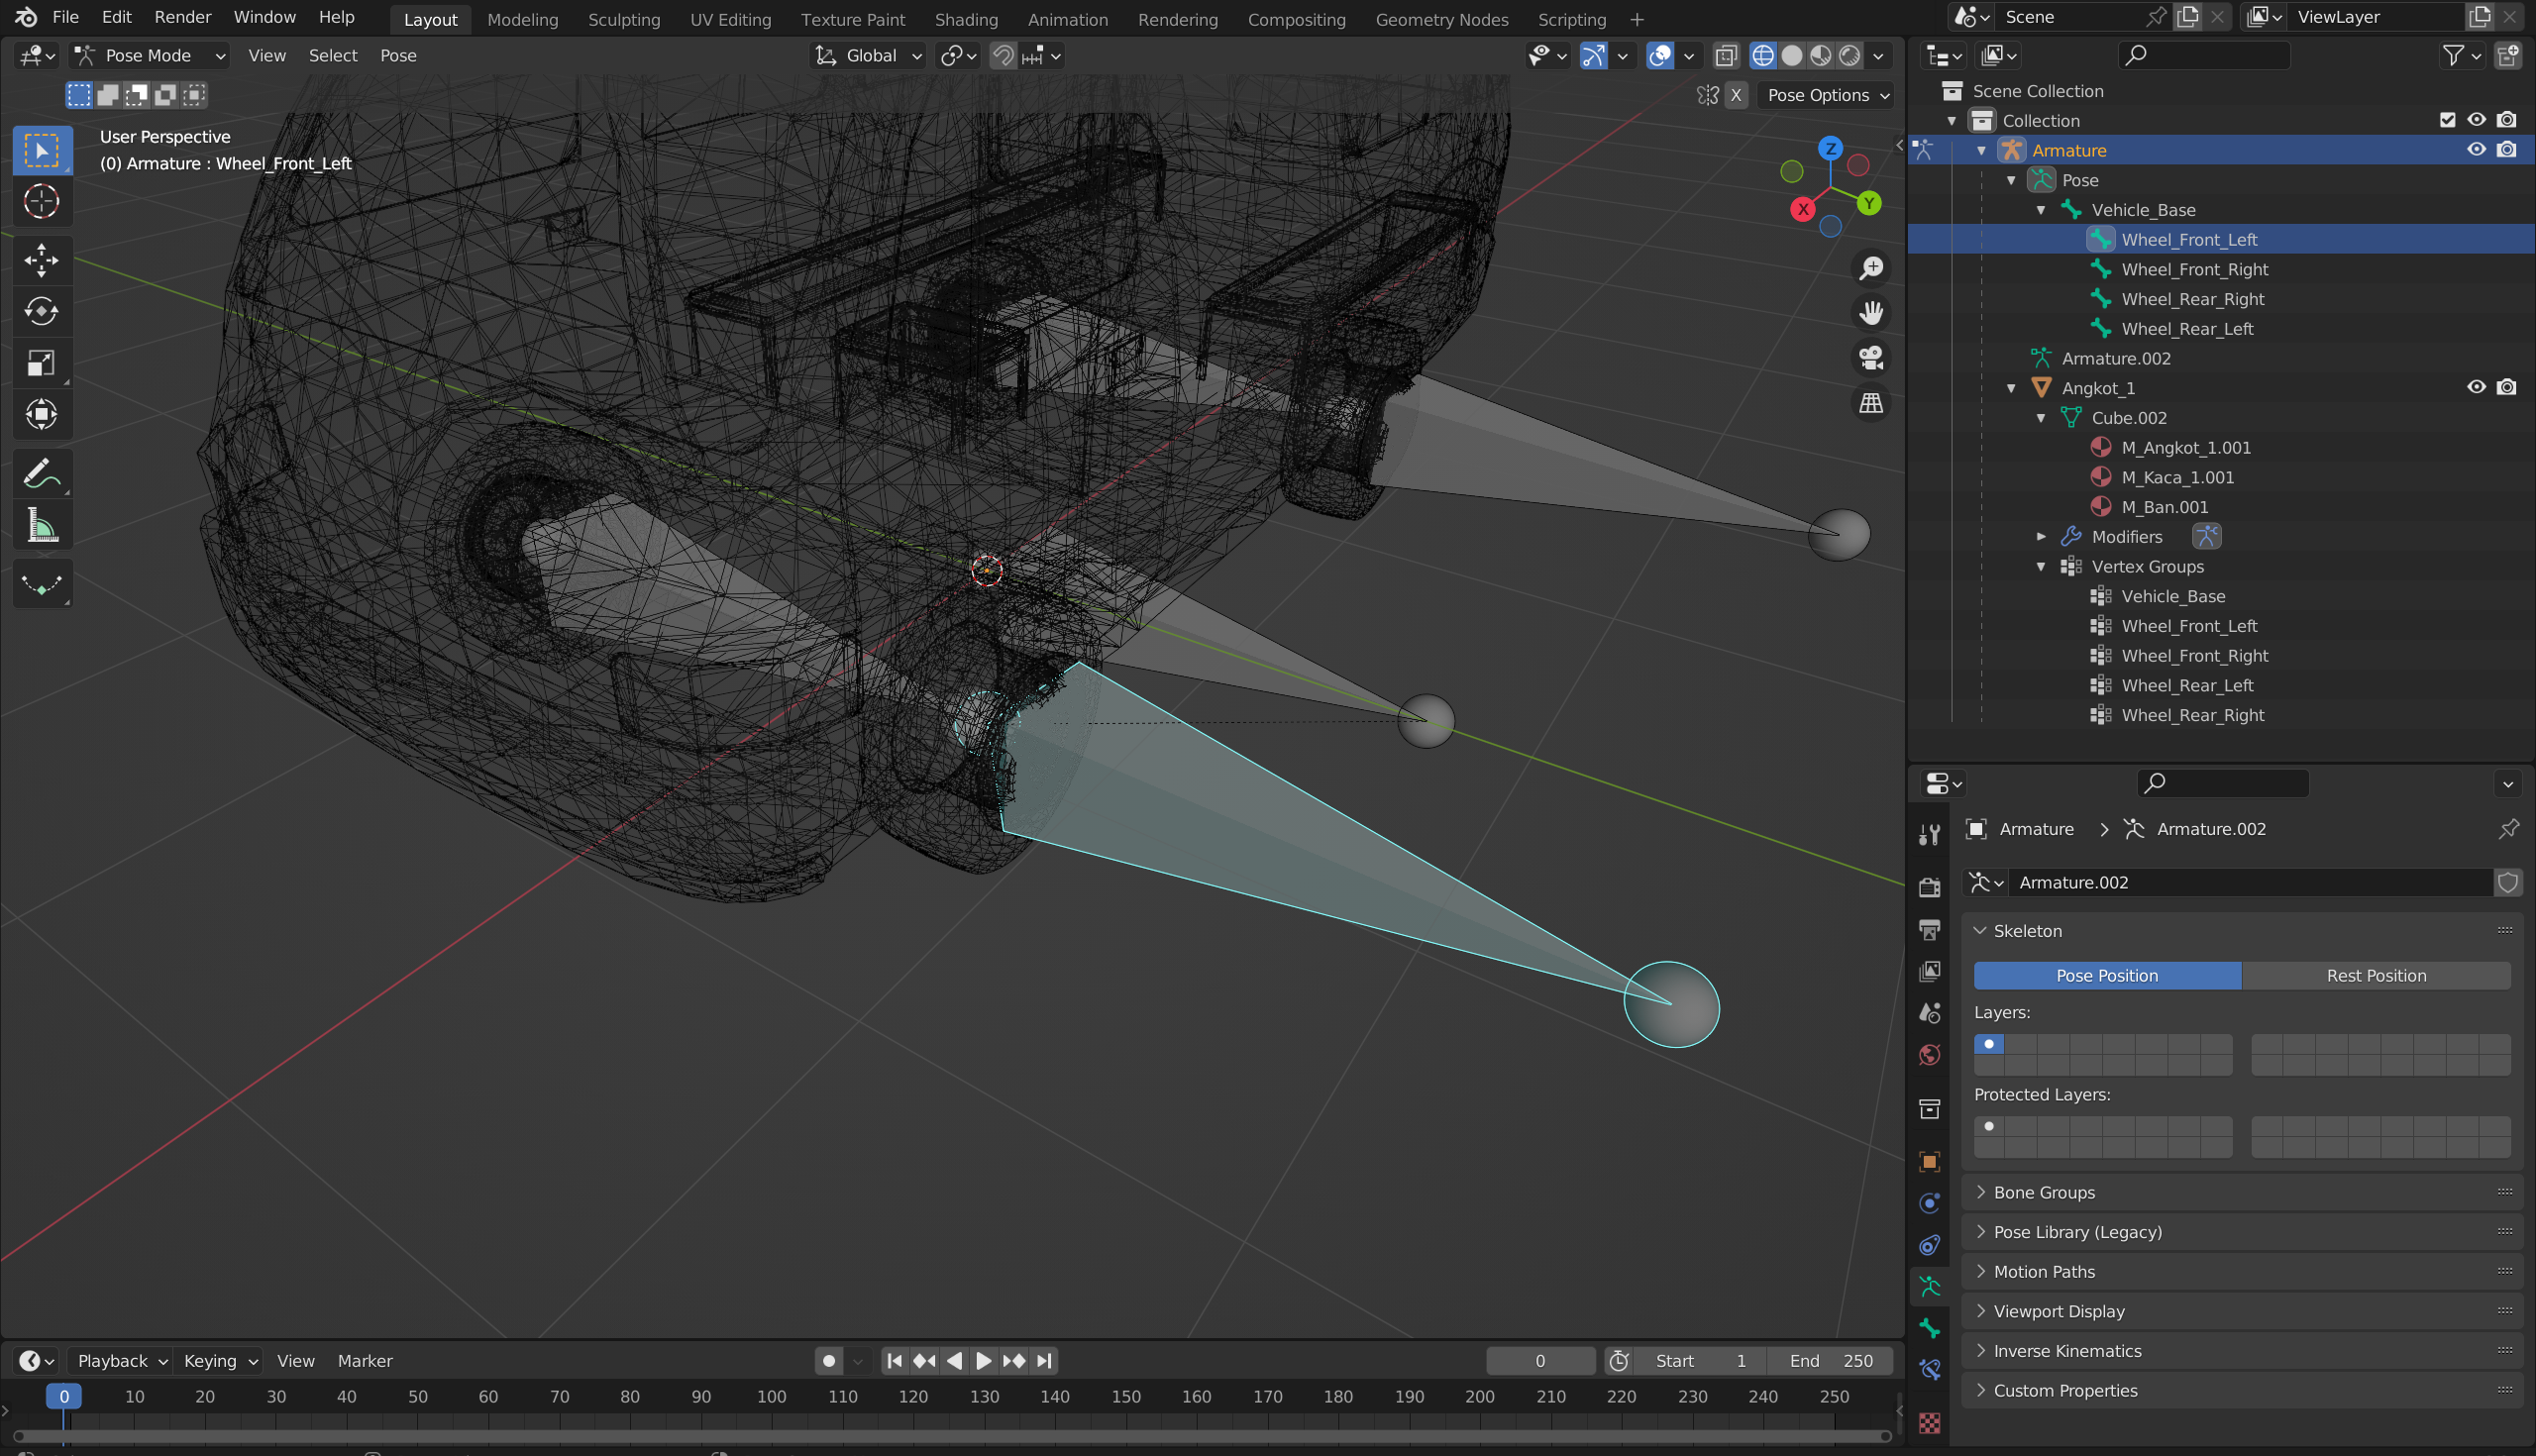
\includegraphics[width=0.4\textwidth]{resources/chapter-4/skinned-wheel-default.png}}
	\hfill
	\subfloat[Perubahan posisi roda]{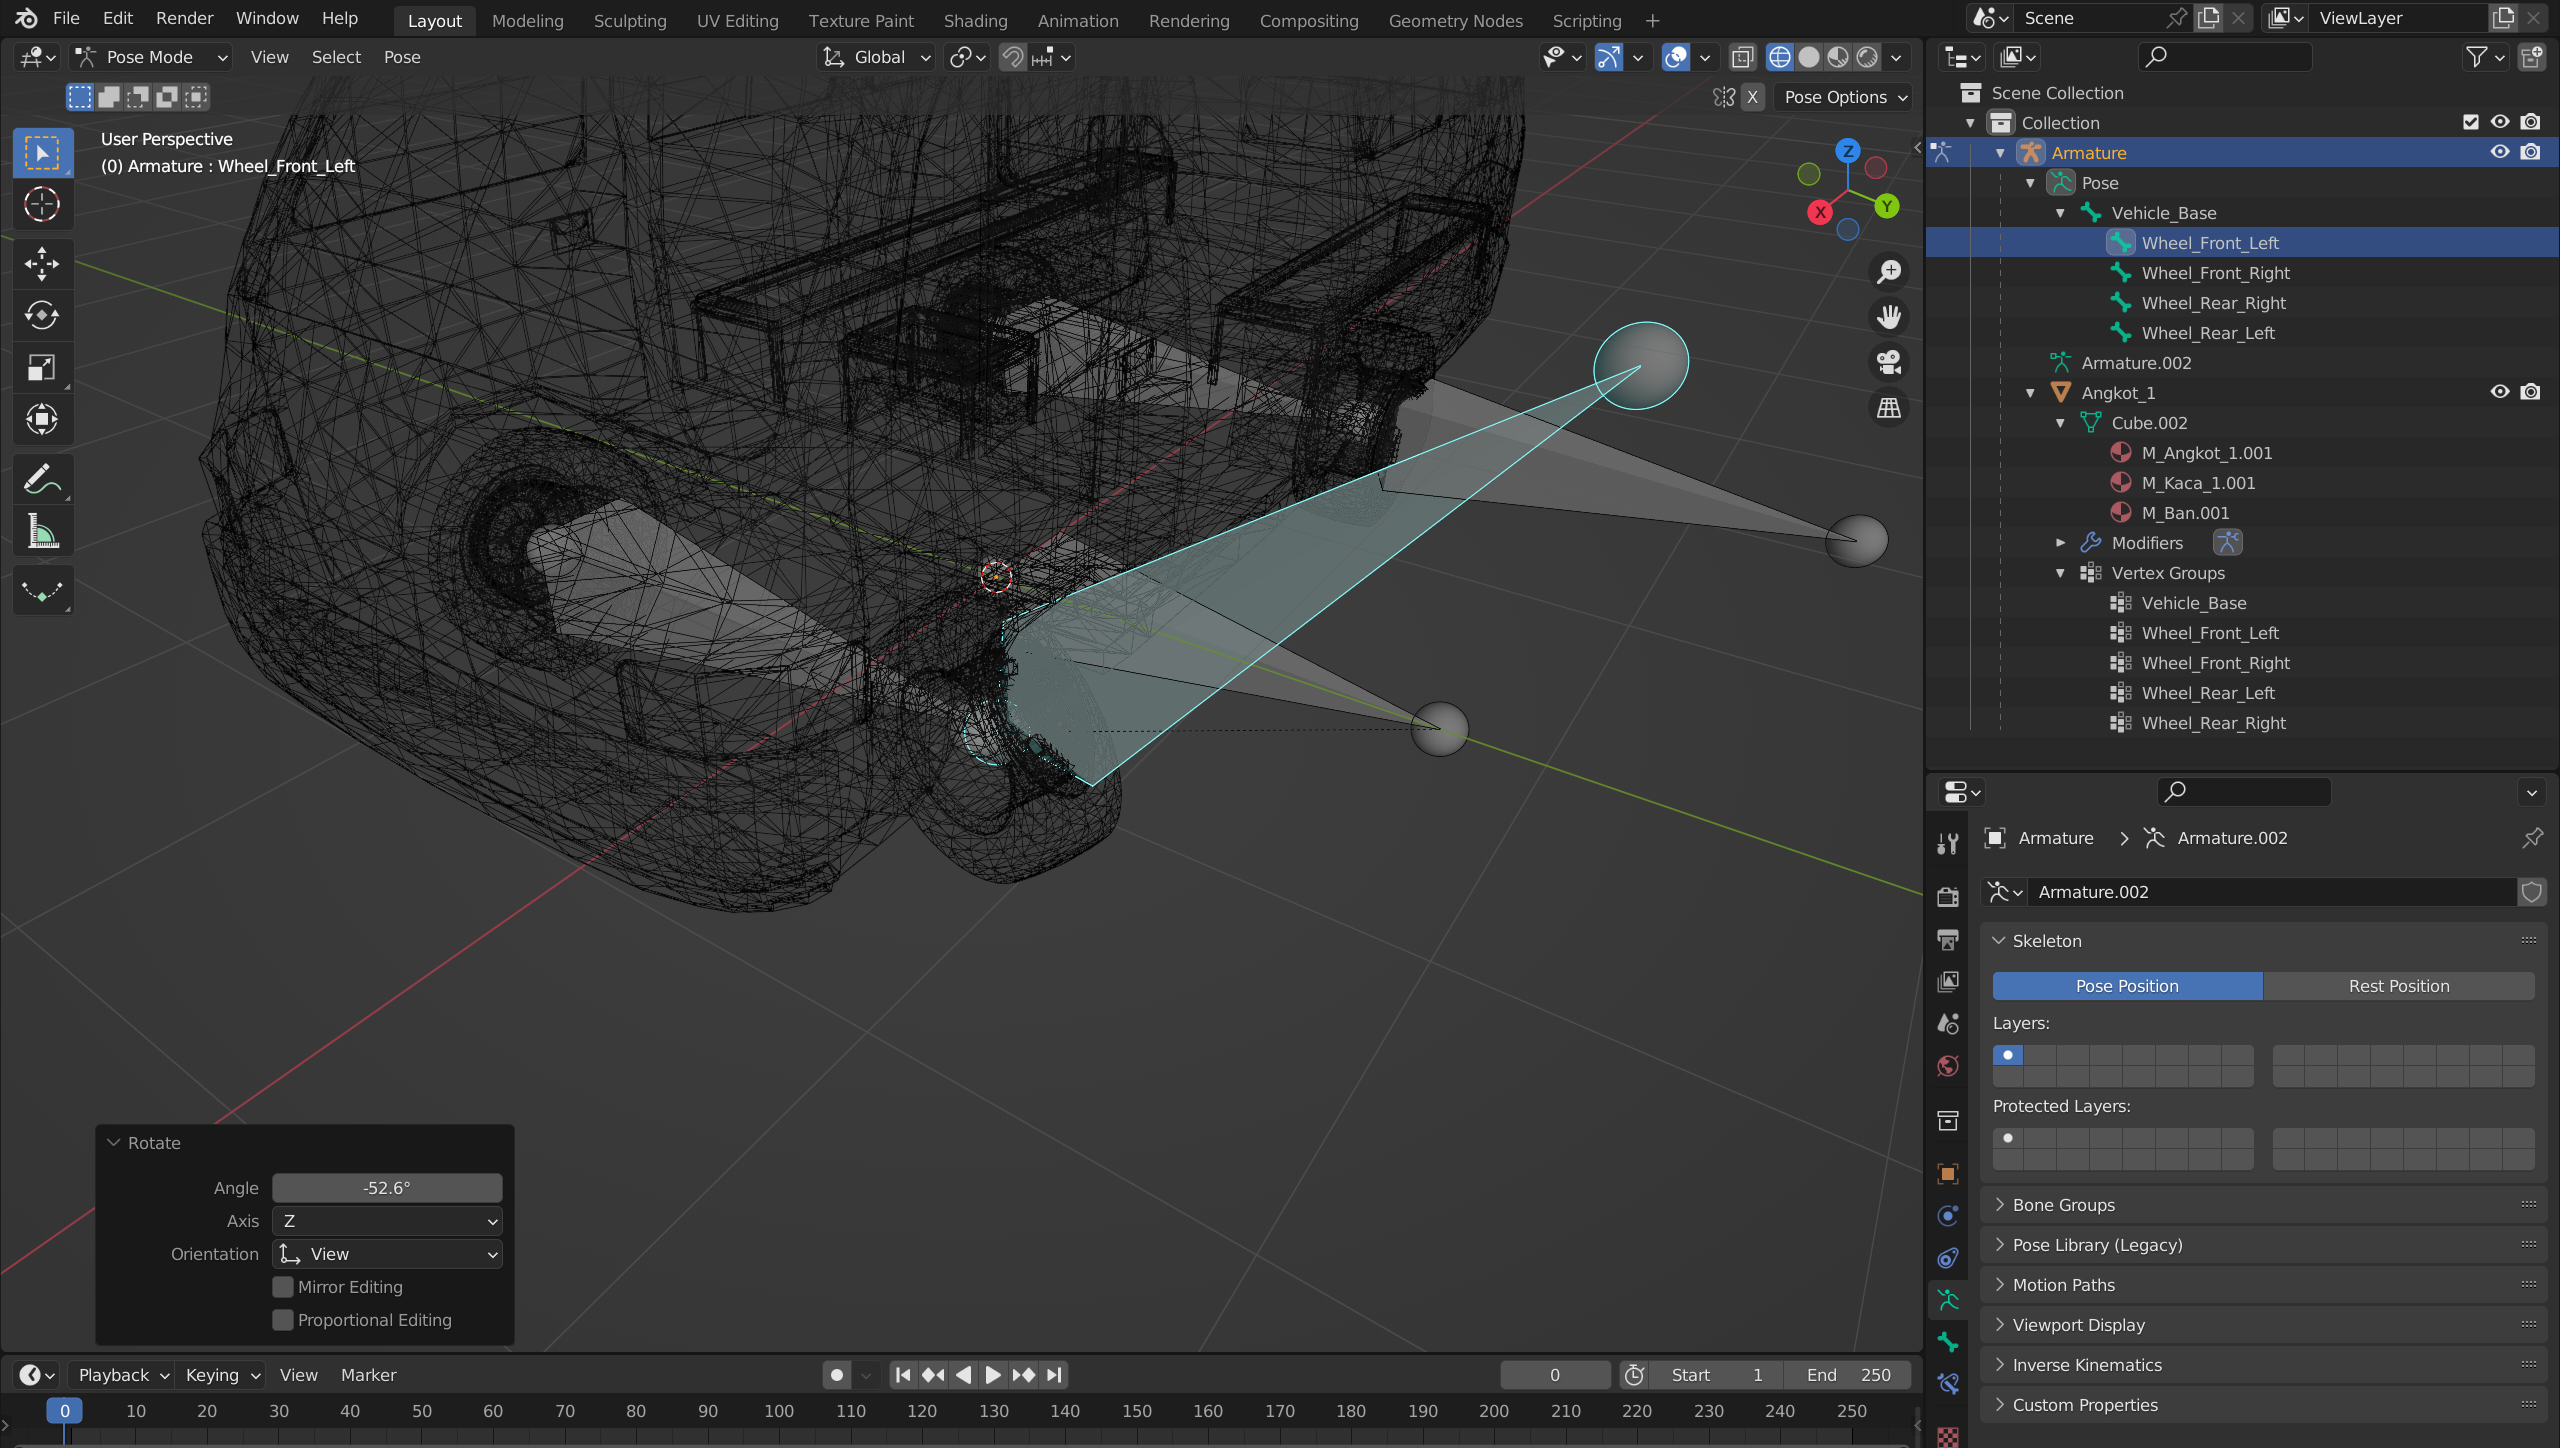
\includegraphics[width=0.4\textwidth]{resources/chapter-4/skinned-wheel-moved.png}}
	\caption{Hasil \textit{skinning} roda yang benar}
	\label{fig:wheel-skinning}
\end{figure}

Aset model 3D dapat diekspor ke dalam format FBX dengan cara memilih pilihan
pada Gambar \ref{fig:export-fbx}.

\begin{figure}[ht]
	\centering
	\subfloat[Opsi ekspor FBX]{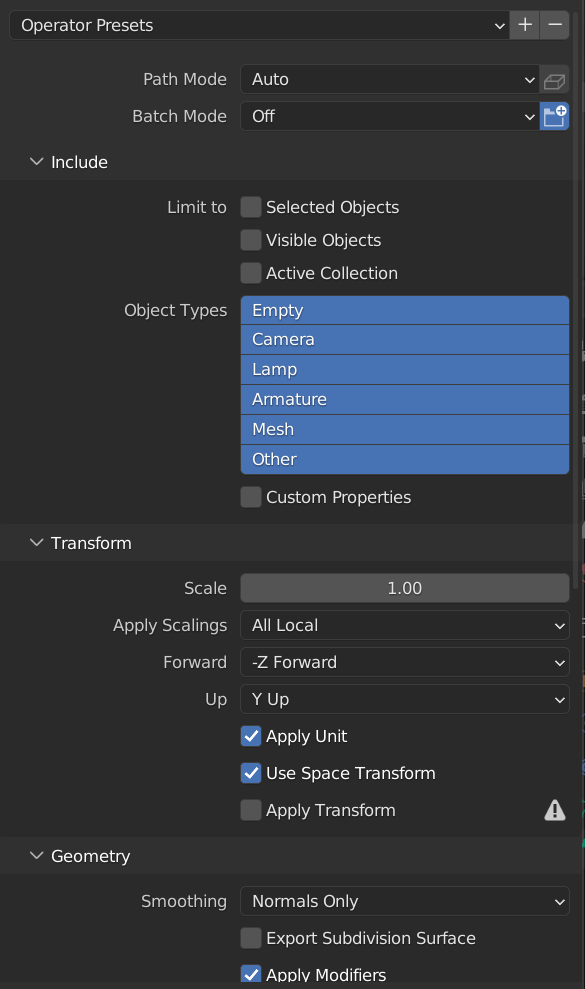
\includegraphics[width=0.4\textwidth]{resources/chapter-4/export-fbx-options-1.png}}
	\hfill
	\subfloat[Opsi ekspor FBX lanjutan]{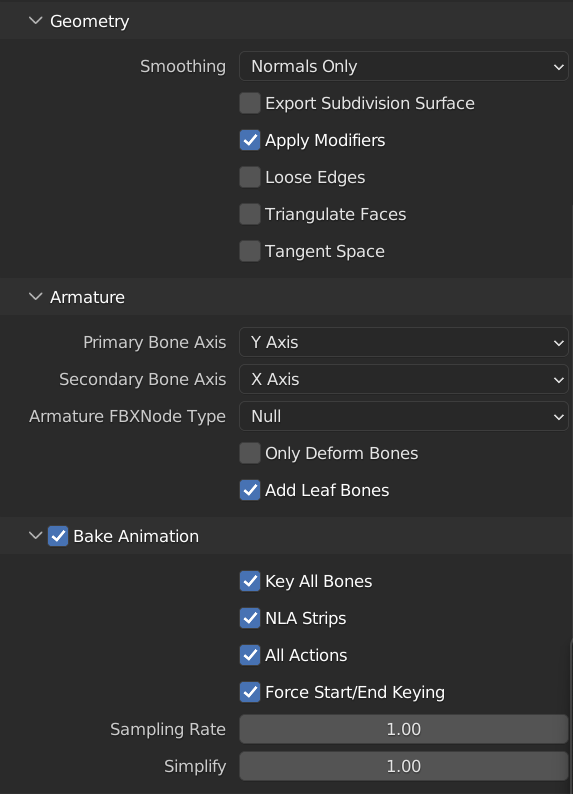
\includegraphics[width=0.4\textwidth]{resources/chapter-4/export-fbx-options-2.png}}
	\caption{Opsi ekspor FBX}
	\label{fig:export-fbx}
\end{figure}

\subsubsection{Impor Berkas FBX ke CARLAUE4}

\dots

% TODO: trouble shooting? hal2 yang harus diperhatikan

% TODO:
% navigate
% new folder
% import + options
% make static mesh buat ganti ...
% set physical asset mesh
% buat animation blueprint

% navigate ke bp folder
% buat folder baru
% buat bp roda, bp kendaraan + configs

% add dto vehicle factory

% spawn vehicle (implemented but does it work?)


% \section{Sepeda Onthel, Sepeda Motor, dan Becak}
% \subsection{Pembuatan Aset Model 3D untuk Ekspor FBX}
% \subsubsection{Impor Berkas FBX ke CARLAUE4}

Gambar \ref{fig:tram-carla} menunjukkan hasil implementasi trem. Gambar
\ref{fig:angkot-carla} menunjukkan hasil implementasi trem  angkot.

\begin{figure}[ht]
    \centering
    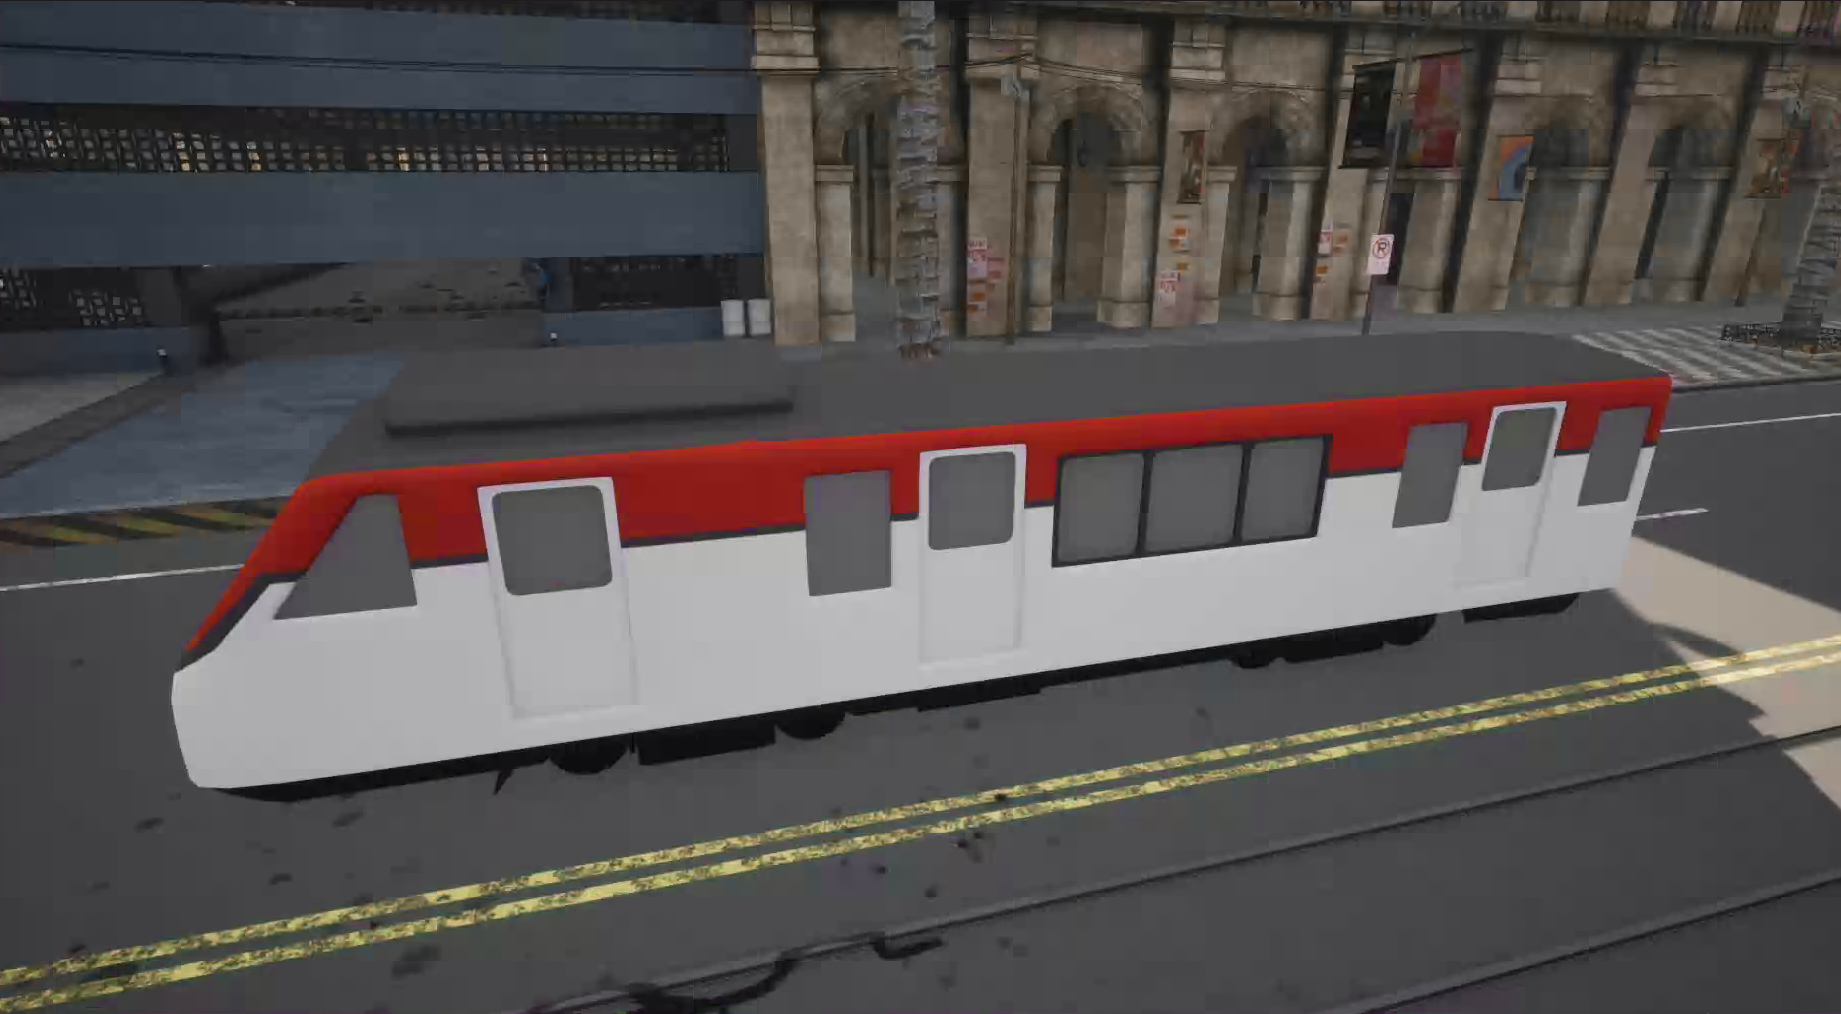
\includegraphics[width=0.6\textwidth]{resources/chapter-4/tram-carla.png}
    \caption{Implementasi trem dalam lingkungan simulasi}
    \label{fig:tram-carla}
\end{figure}

\begin{figure}[ht]
    \centering
    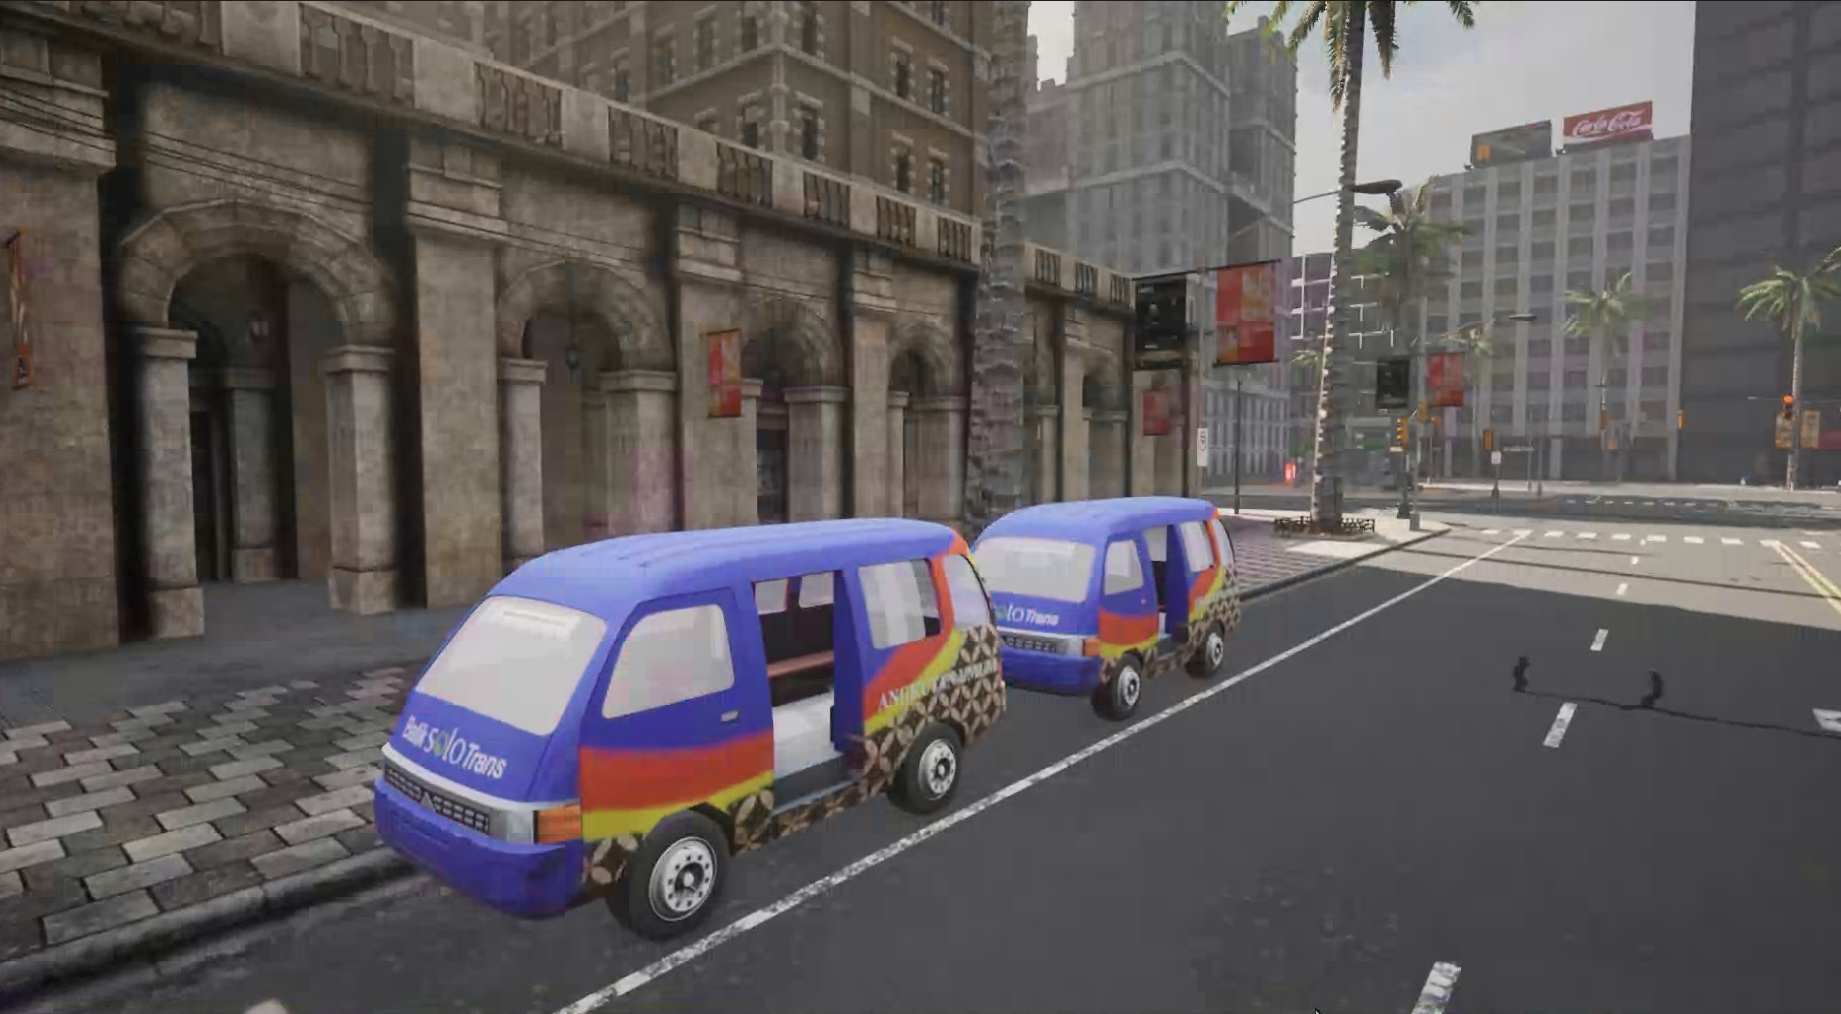
\includegraphics[width=0.6\textwidth]{resources/chapter-4/angkot.png}
    \caption{Implementasi angkot dalam lingkungan simulasi}
    \label{fig:angkot-carla}
\end{figure}

\section{Implementasi Lingkungan}

Penambahan aset model 3D ke dalam lingkungan simulasi dilakukan dengan membuat
folder baru pada direktori yang bersangkutan kemudian mengimpor aset model 3D ke
dalam folder tersebut. Cara menambahkan objek-objek statis ini adalah dengan
menarik objek dari impor dari \textit{Content Browser} ke dalam \textit{World
Outliner}. Setelah itu, dapat dilakukan penyesuaian skala, posisi, dan rotasi
aset pada \textit{World Outliner}. Penyesuaian lingkungan dapat dilakukan dengan
memilih dan mengaktifkan tingkat atau level objek yang ingin diubah.

% TODO: insert images, add directories, world levels, world outliner kah istilahnya?
% penyesuiannya lingkungan?

\subsection{Stasiun Madiun dan Stasiun Solokota}
Gambar \ref{fig:stasiun-madiun} menunjukkan implementasi model Stasiun Madiun
(lihat Gambar \ref{fig:stasiun-madiun-model}). Model stasiun kemudian
disesuaikan ukurannya dan diposisikan pada ... .

Gambar \ref{fig:stasiun-solokota} menunjukkan implementasi model Stasiun Solokota
(lihat Gambar \ref{fig:stasiun-solokota-model}). Model stasiun kemudian
disesuaikan ukurannya dan diposisikan pada ... .

% TODO: ..., + cara,  ke bab 3?

\begin{figure}[ht]
    \centering
    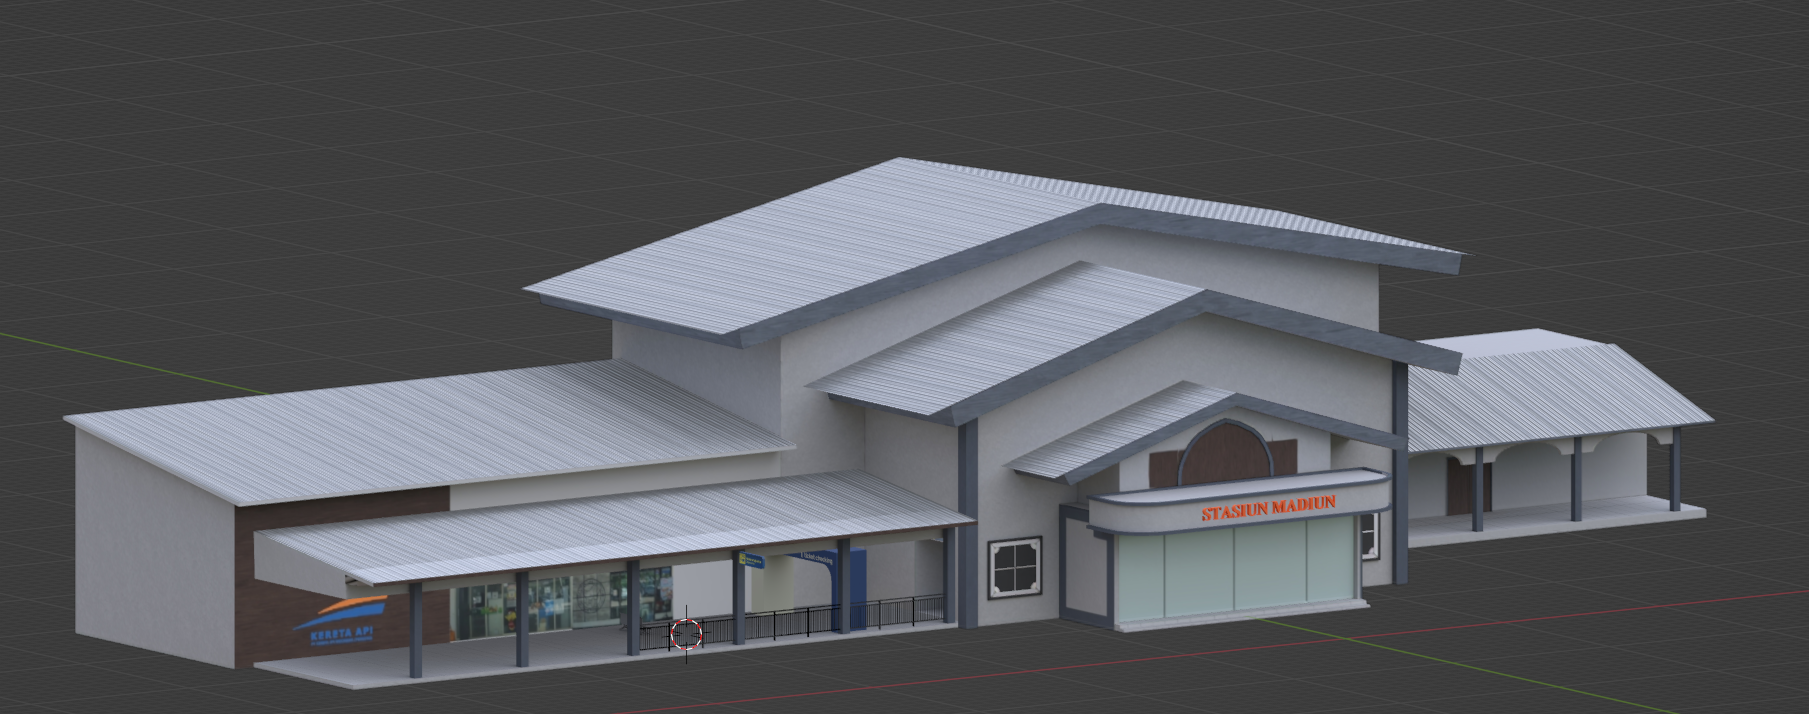
\includegraphics[width=0.6\textwidth]{resources/chapter-3-stasiun-madiun-model.png}
    \caption{Model Stasiun Madiun}
    \label{fig:stasiun-madiun-model}
\end{figure}

\begin{figure}[ht]
    \centering
    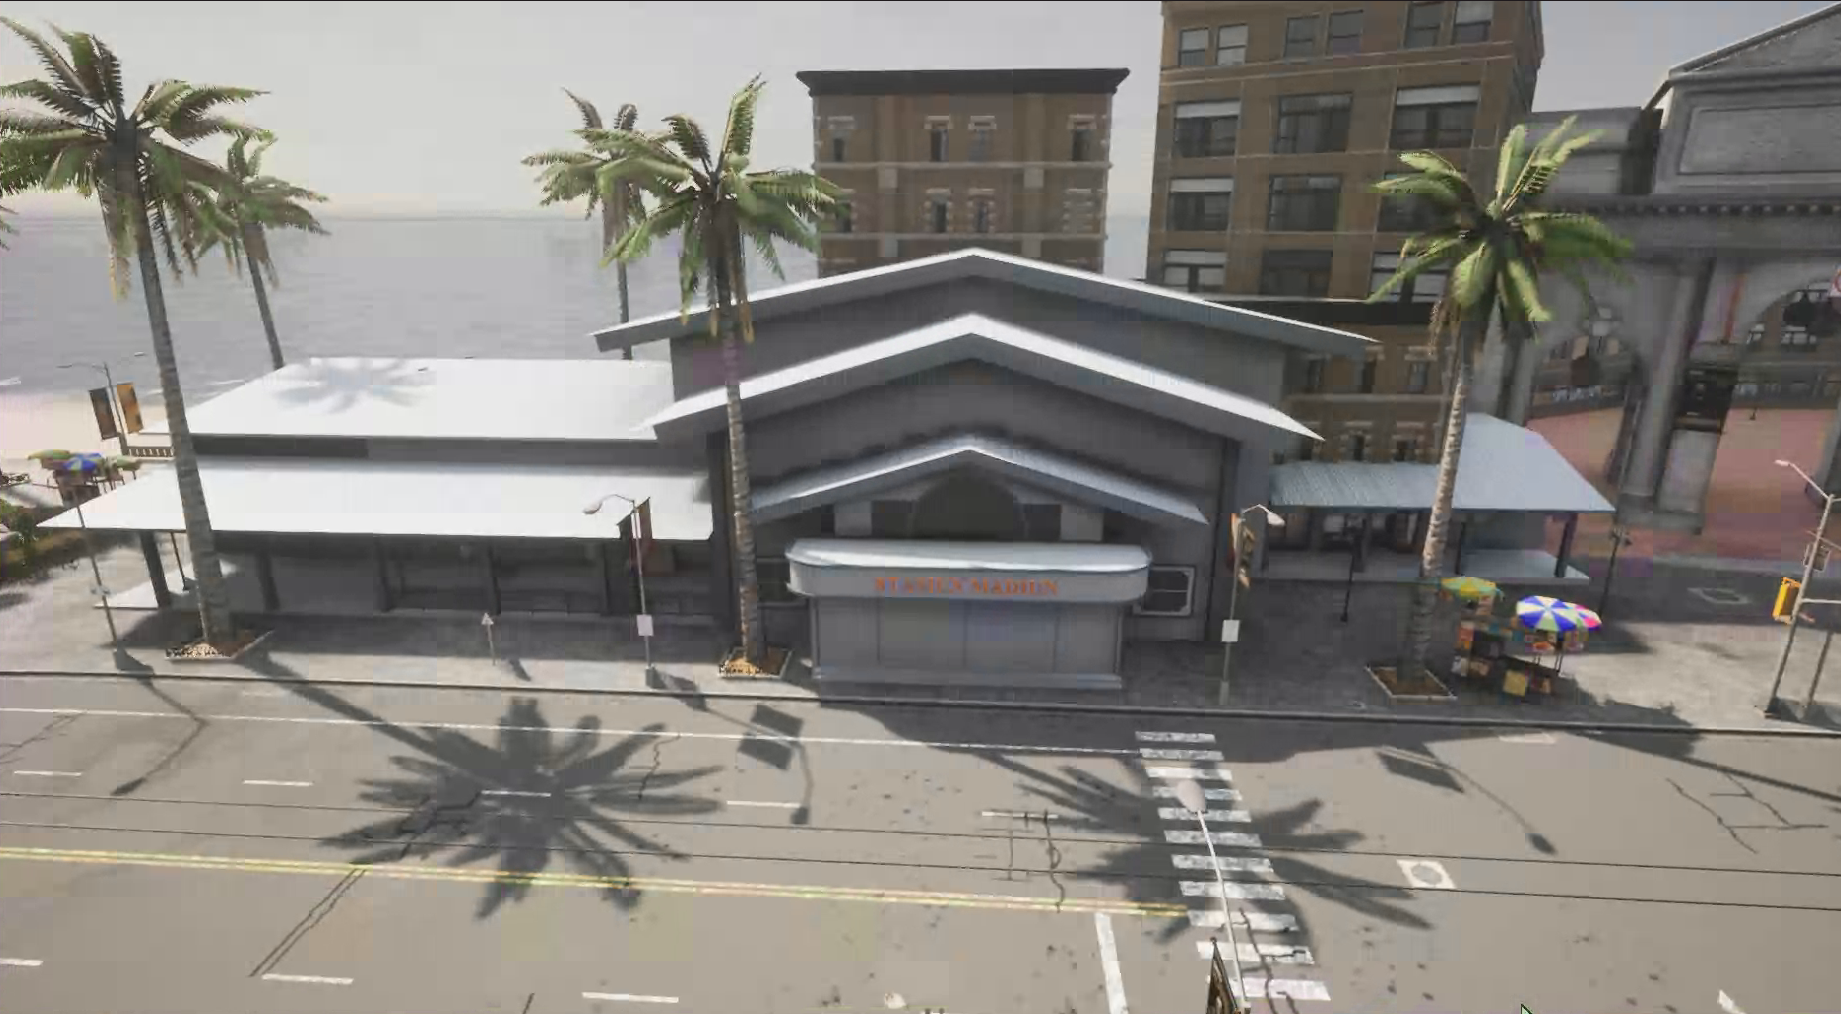
\includegraphics[width=0.6\textwidth]{resources/chapter-4/stasiun-madiun-carla.png}
    \caption{Implementasi stasiun Madiun dalam lingkungan simulasi}
    \label{fig:stasiun-madiun}
\end{figure}

\begin{figure}[ht]
    \centering
    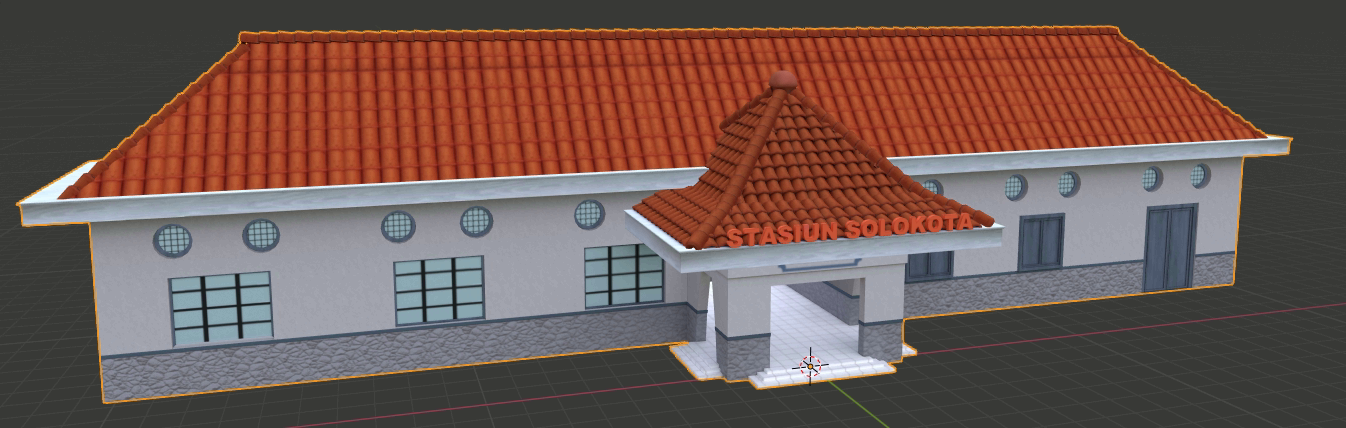
\includegraphics[width=0.6\textwidth]{resources/chapter-3-stasiun-solokota-model.png}
    \caption{Model Stasiun Solokota}
    \label{fig:stasiun-solokota-model}
\end{figure}

\begin{figure}[ht]
    \centering
    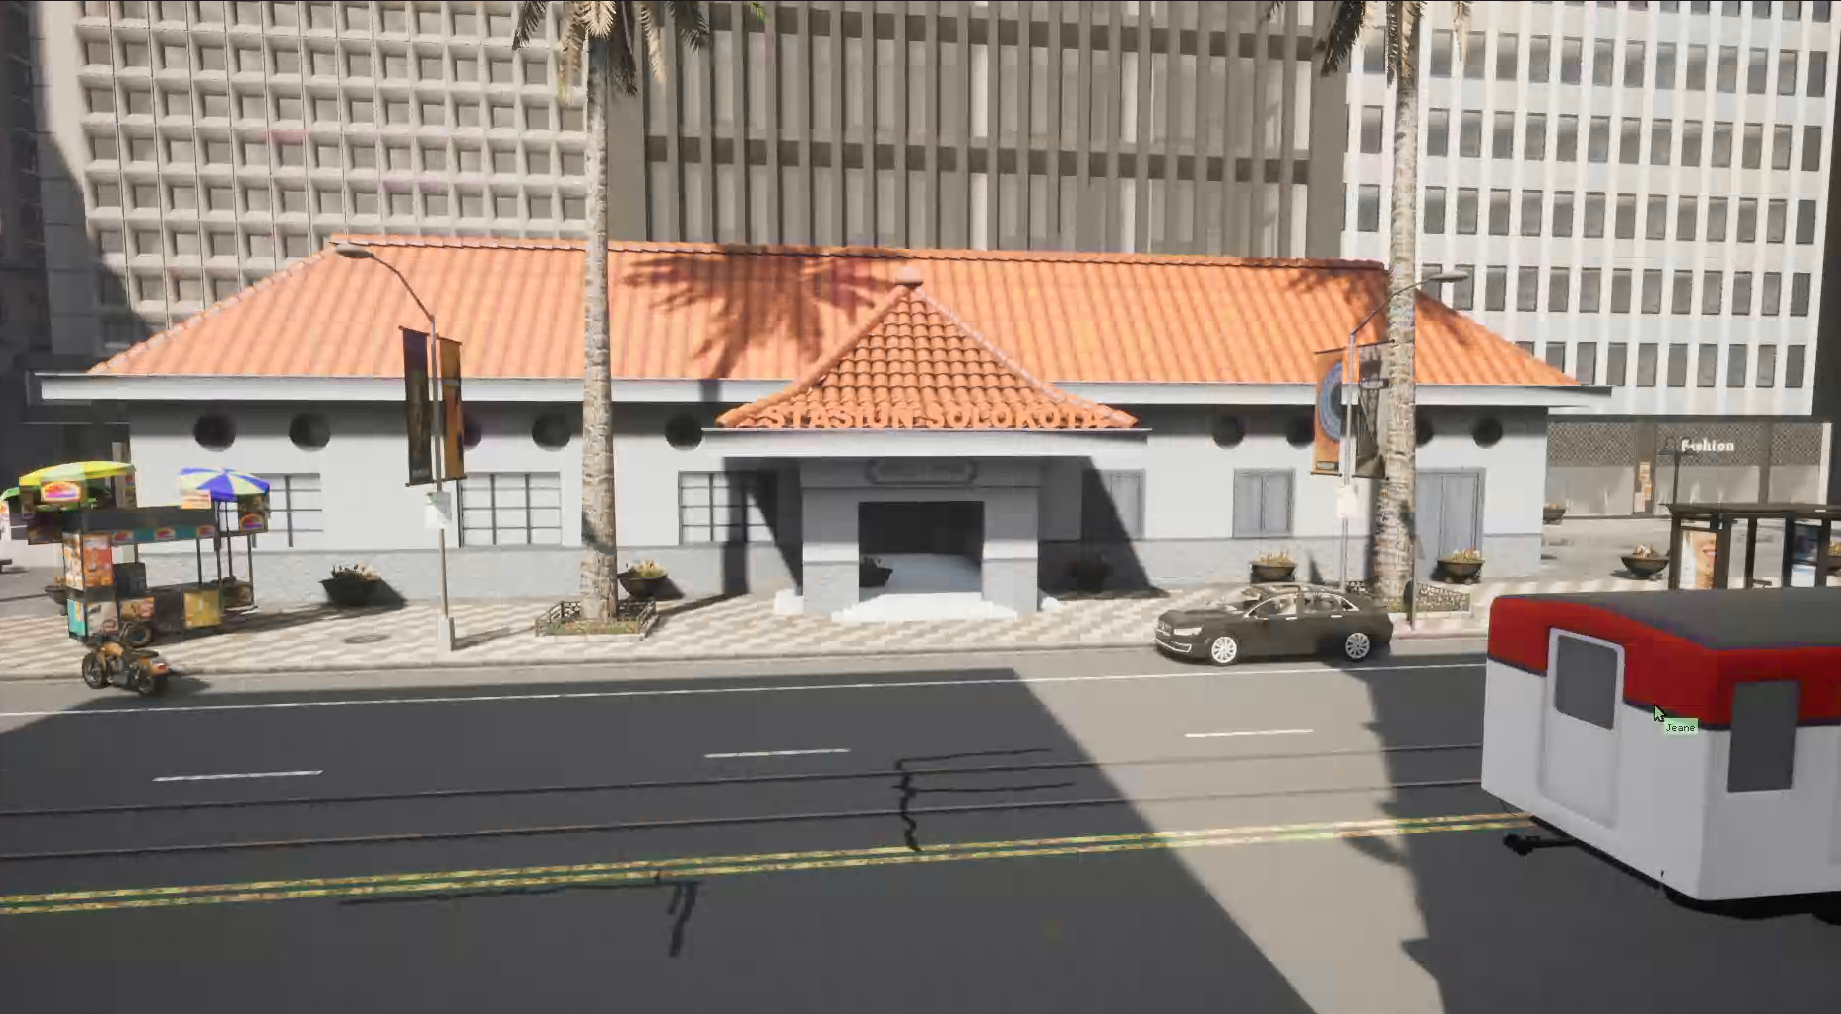
\includegraphics[width=0.6\textwidth]{resources/chapter-4/stasiun-solokota-carla.png}
    \caption{Implementasi stasiun Solokota dalam lingkungan simulasi}
    \label{fig:stasiun-solokota}
\end{figure}

\subsection{Rambu-rambu Lalu Lintas}

\begin{figure}[ht]
	\centering
	\subfloat[]{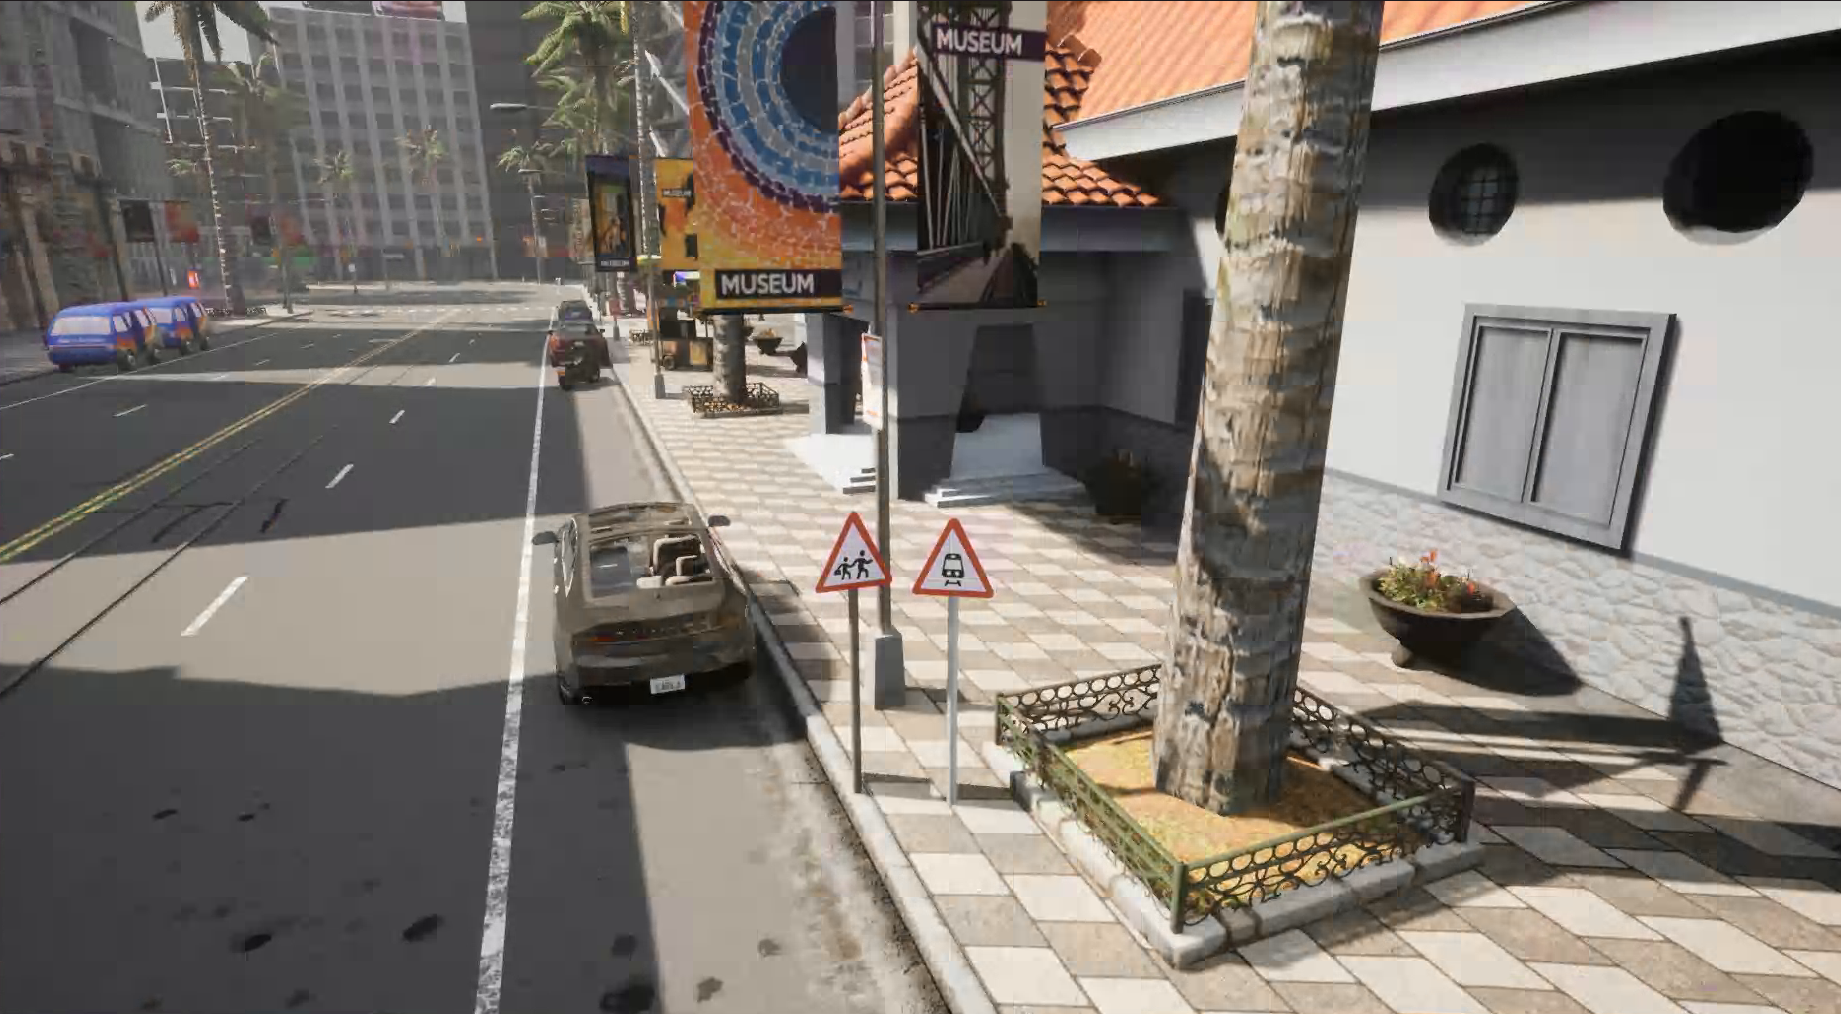
\includegraphics[width=0.4\textwidth]{resources/chapter-4/rambu-1.png}}
	\hfill
	\subfloat[]{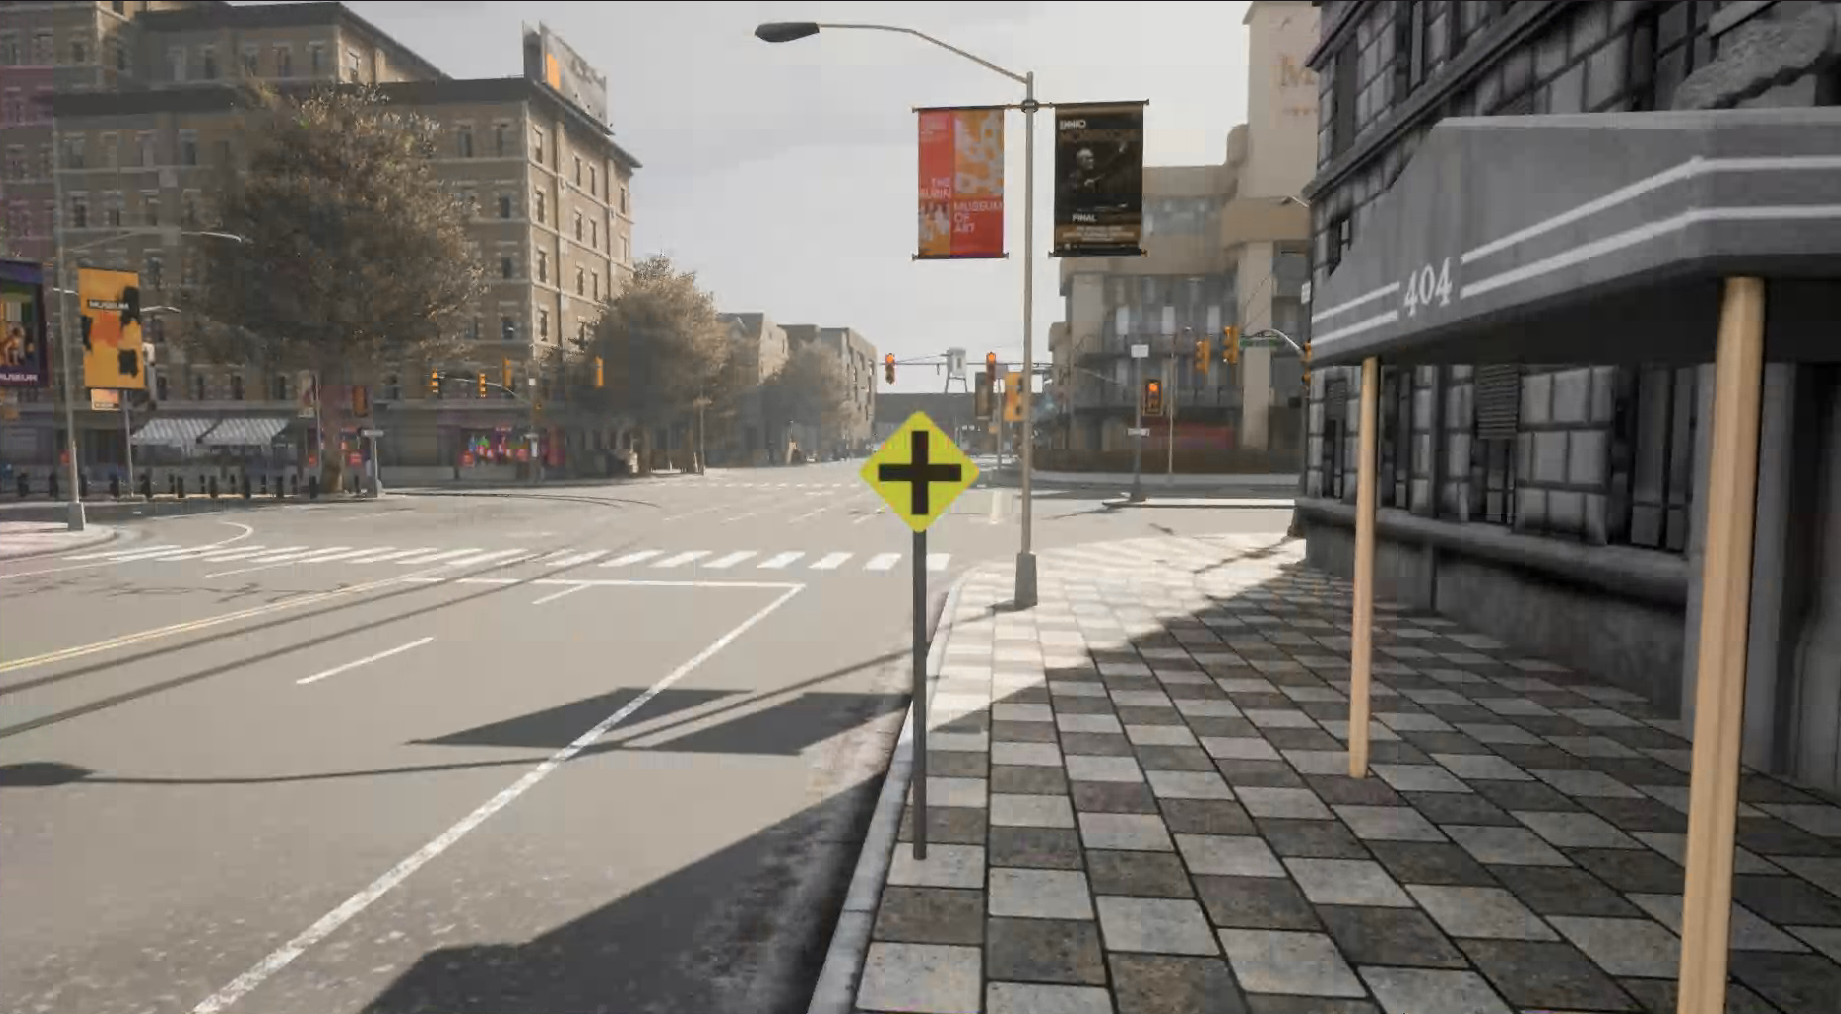
\includegraphics[width=0.4\textwidth]{resources/chapter-4/rambu-2.png}}
	\caption{Implementasi rambu-rambu lalu lintas dalam lingkungan simulasi}
	\label{fig:road-signs}
\end{figure}

\subsection{Rel}
% import mesh sebagai objek statis
% spline: butuh banyak edge/verts
% topview + stasiun

Gambar \ref{fig:rel} dan Gambar \ref{fig:rel-2} menunjukkan implementasi rel.

% rel (lihat Gambar \ref{fig:rel-model}).

% \begin{figure}[ht]
%     \centering
%     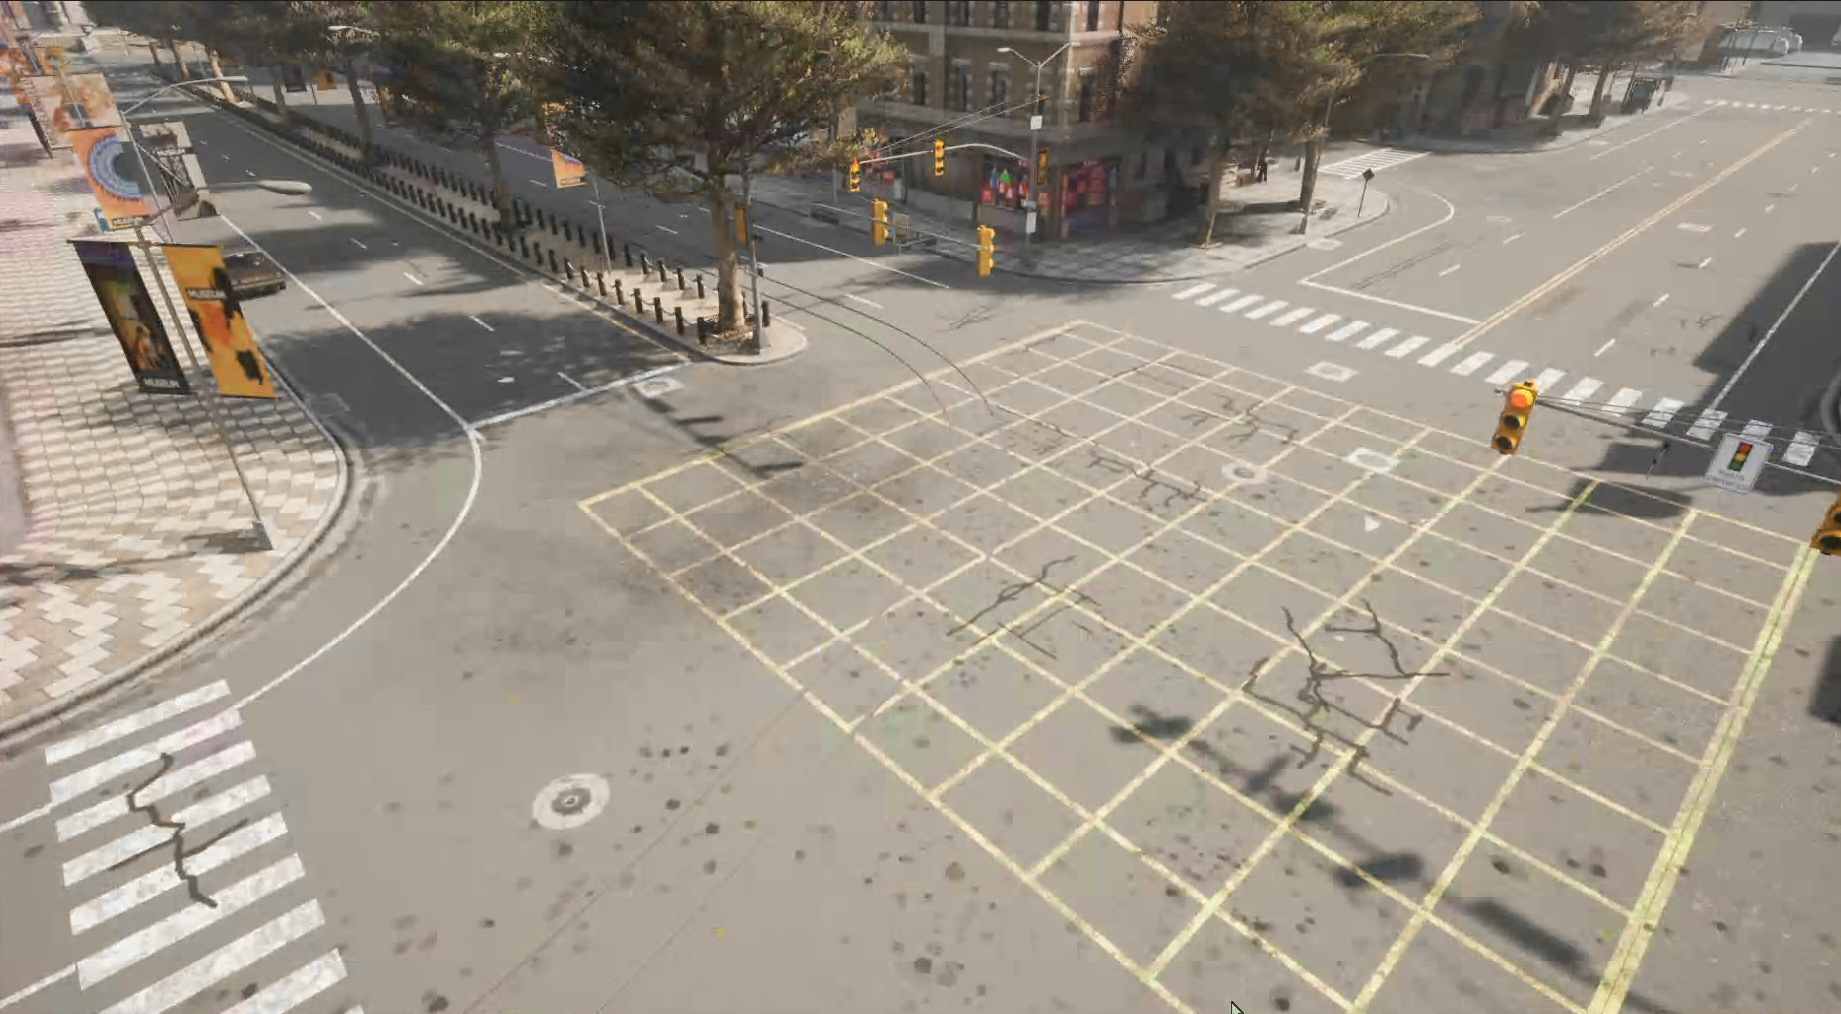
\includegraphics[width=0.6\textwidth]{resources/chapter-4/rel.png}
%     \caption{Implementasi rel dalam lingkungan simulasi}
%     \label{fig:rel-model}
% \end{figure}

\begin{figure}[ht]
    \centering
    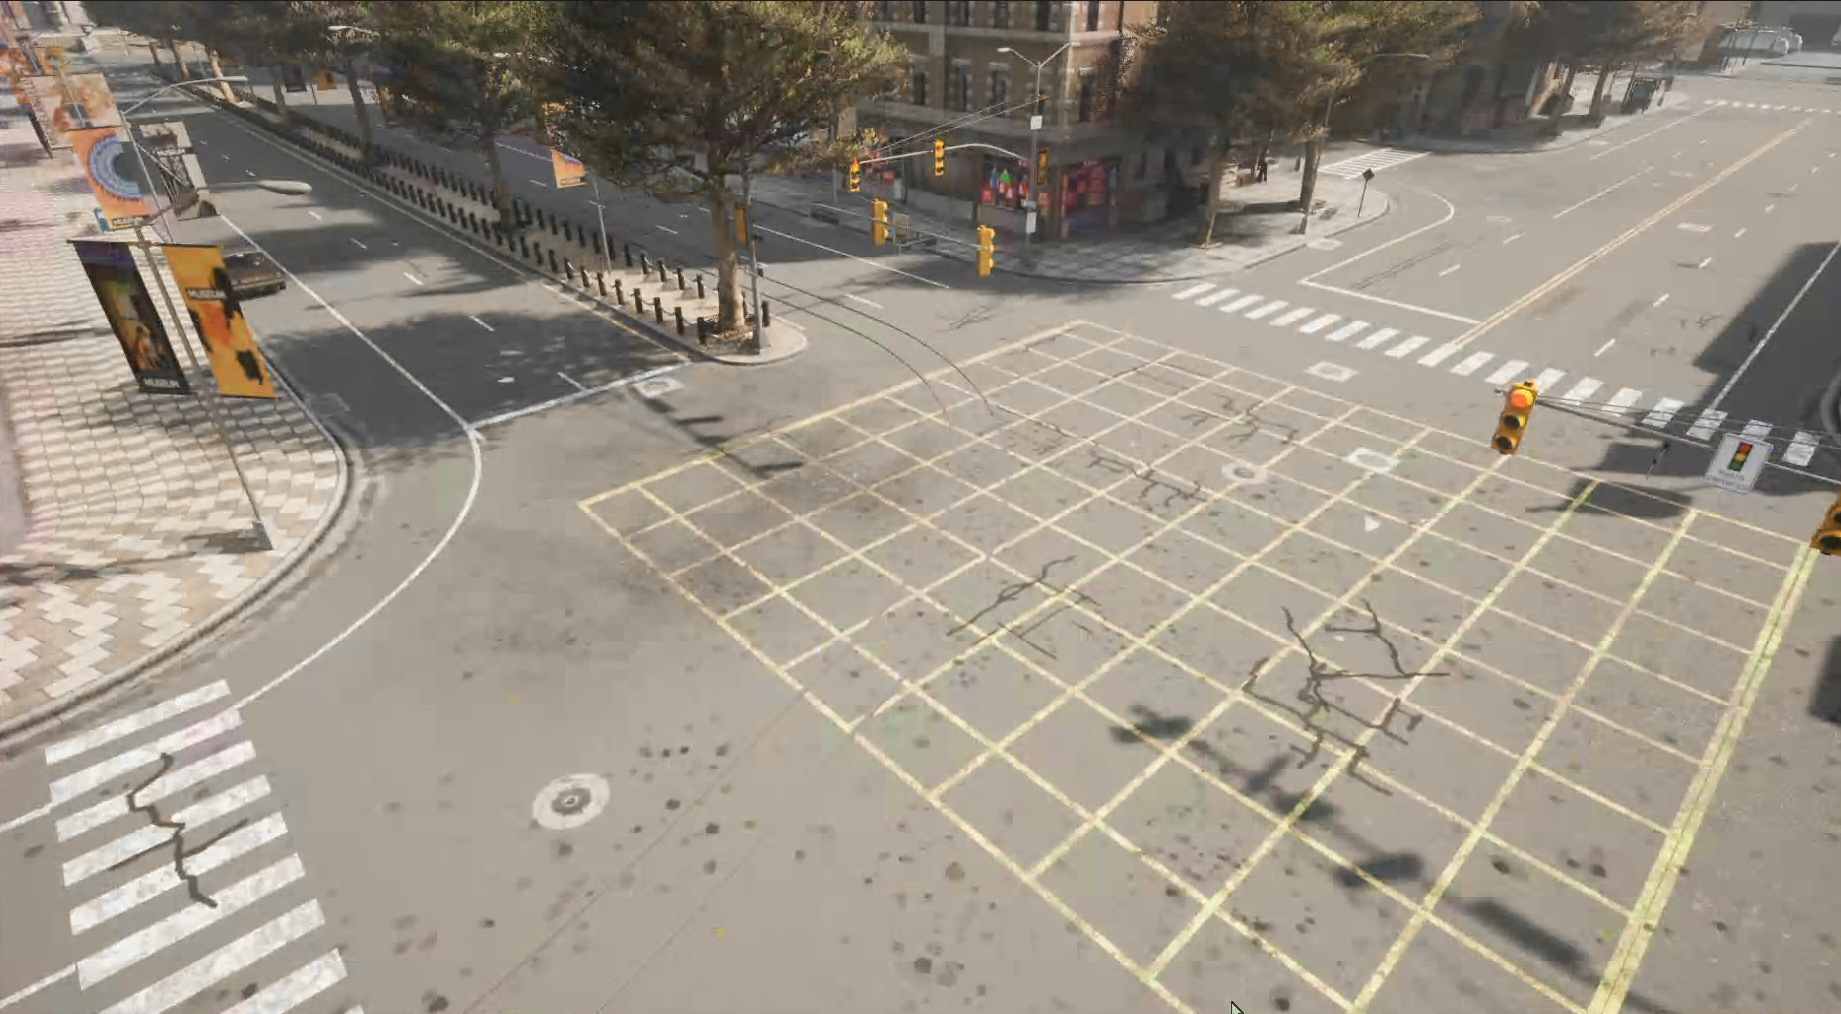
\includegraphics[width=0.6\textwidth]{resources/chapter-4/rel.png}
    \caption{Implementasi rel dalam lingkungan simulasi}
    \label{fig:rel}
\end{figure}

\begin{figure}[ht]
    \centering
    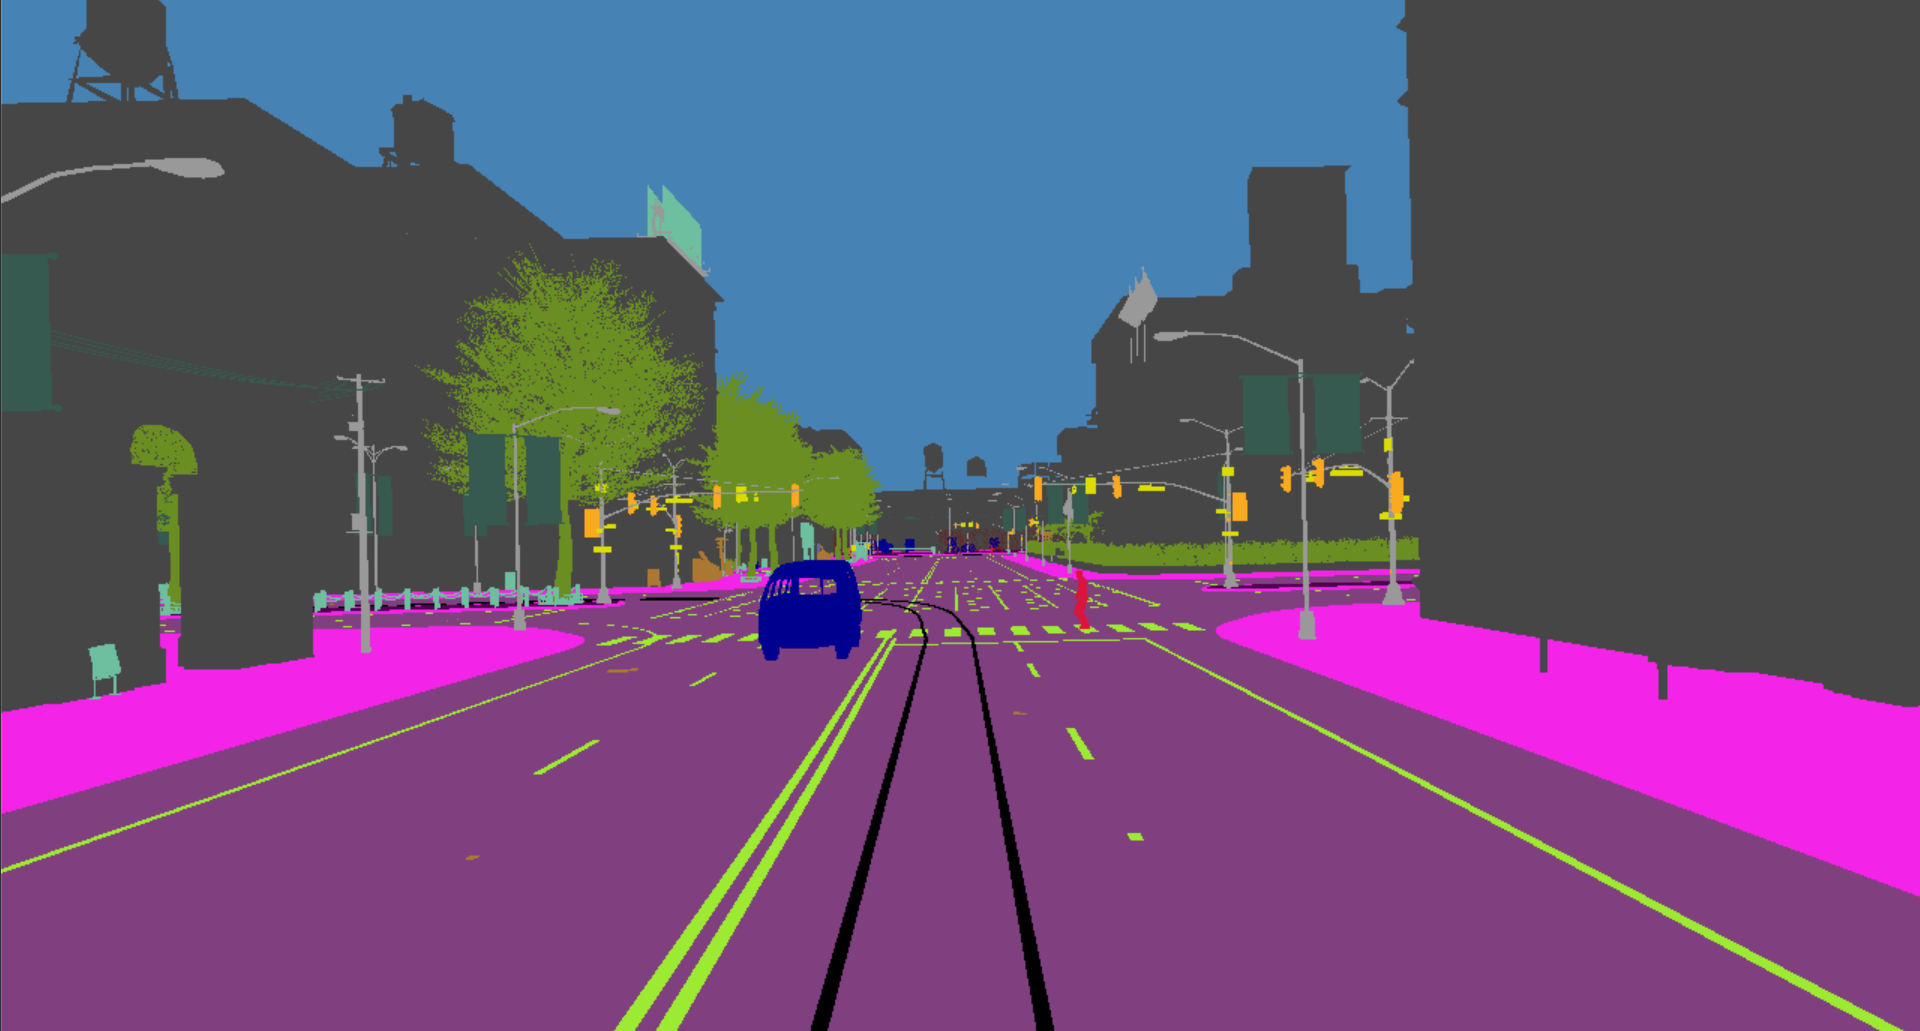
\includegraphics[width=0.6\textwidth]{resources/chapter-4/rel-segmentation-camera.png}
    \caption{Implementasi rel dalam lingkungan simulasi (tampilan segmentasi semantik)}
    \label{fig:rel-2}
\end{figure}

\section{Validasi}

\subsection{Tujuan Validasi}

Tujuan validasi adalah untuk memastikan bahwa objek2 berperilaku normal (seperti
aslinya) dan stabil saat simulasi berjalan.

% TODO:

\subsection{Hasil Validasi}
% manual + generate

\section{Evaluasi}
% kendaraan roda 2 dan 3 berhasil diimplementasikan namun tidak stabil
